% Working Title: hesse: Tracking Loss-Landscape Curvature Through Training, and the Edge of Stability Beyond Gradient Descent
% Alternative Title 1: Beyond the Edge: Matrix-Free Curvature Dynamics and Stability Limits in Deep Learning
% Alternative Title 2: Tracking Curvature in Deep Learning: An Empirical Study of the Edge of Stability Across Optimizers and Architectures

\documentclass[10pt,twocolumn]{article}
\usepackage[margin=0.75in]{geometry}
\usepackage{amsmath,amssymb,amsfonts,amsthm}
\usepackage{booktabs}
\usepackage{graphicx}
\usepackage{microtype}
\usepackage{hyperref}
\usepackage{xcolor}
\usepackage{cite}
\usepackage{subcaption}
\usepackage{tabularx}
\usepackage{enumitem}
\setlist{noitemsep,topsep=2pt,parsep=0pt,partopsep=0pt}

\renewcommand{\topfraction}{0.95}
\renewcommand{\bottomfraction}{0.85}
\renewcommand{\textfraction}{0.05}
\renewcommand{\floatpagefraction}{0.85}

\setlength{\textfloatsep}{7pt plus 2pt minus 2pt}
\setlength{\floatsep}{5pt plus 2pt minus 2pt}
\setlength{\intextsep}{5pt plus 2pt minus 2pt}
\setlength{\abovecaptionskip}{4pt}
\setlength{\belowcaptionskip}{3pt}

\makeatletter
\renewcommand\section{\@startsection {section}{1}{\z@}%
                                   {-1.8ex \@plus -0.4ex \@minus -.2ex}%
                                   {0.8ex \@plus .2ex}%
                                   {\normalfont\large\bfseries}}
\renewcommand\subsection{\@startsection{subsection}{2}{\z@}%
                                     {-1.3ex\@plus -0.3ex \@minus -.2ex}%
                                     {0.6ex \@plus .2ex}%
                                     {\normalfont\normalsize\bfseries}}
\makeatother

\let\oldbibliography\thebibliography
\renewcommand{\thebibliography}[1]{%
  \oldbibliography{#1}%
  \small
  \setlength{\itemsep}{0pt plus 0.2ex}%
  \setlength{\parsep}{0pt}%
}

\hypersetup{
    colorlinks=true,
    linkcolor=blue!70!black,
    citecolor=blue!70!black,
    urlcolor=blue!70!black
}

\title{\textbf{\texttt{hesse}: Tracking Loss-Landscape Curvature Through Training,\\and the Edge of Stability Beyond Gradient Descent}}

\author{
    \textbf{Aditya Surse}\\
    Independent Researcher\\
    \texttt{adityasurse42@gmail.com}
}

\date{\today}

\begin{document}

\maketitle

\begin{abstract}
Understanding non-convex loss-landscape geometry is central to explaining optimization and generalization in deep learning. While classical optimization assumes descent within linear stability boundaries ($\eta \le 2/\lambda_{\max}$), recent theory identifies an ``Edge of Stability'' (EoS) regime where gradient descent operates persistently at the boundary. However, empirical tooling has predominantly remained post-hoc or restricted to simple gradient descent. We introduce \texttt{hesse}, an open-source, matrix-free Hessian computation and telemetry library that instruments neural network training with zero-overhead curvature tracking. We deploy \texttt{hesse} across six systematic benchmarks spanning 21 configurations ($S \in \{42, 43, 44\}$). In full-batch gradient descent ($\eta=0.1$), we reproduce EoS dynamics, with sharpness reaching a plateau ratio of $0.962 \pm 0.001$ of $2/\eta=20.0$. In stochastic gradient descent, small batch sizes ($B=32$) suppress sharpness to $24.65 \pm 0.00$ while driving non-monotonic loss transitions to $55.2\%$. Under Adam, coordinate-wise preconditioning breaks the scalar ceiling, yielding preconditioned ratios exceeding $85{,}601 \pm 37{,}554$. For Lion, sign updates constrain step magnitudes globally, bounding directional curvature $\kappa_{\text{sign}}$ from $0.037$ to $0.005$ without divergence. Finally, Vision Transformers exhibit pronounced spectral gaps ($\lambda_1 - \lambda_2 = 11.60$) over convolutional networks ($0.06$).
\end{abstract}

% Float 1 declared early on Page 1 to appear at the top of Page 2
\begin{figure*}[t]
\centering
\begin{subfigure}[b]{0.62\textwidth}
    \centering
    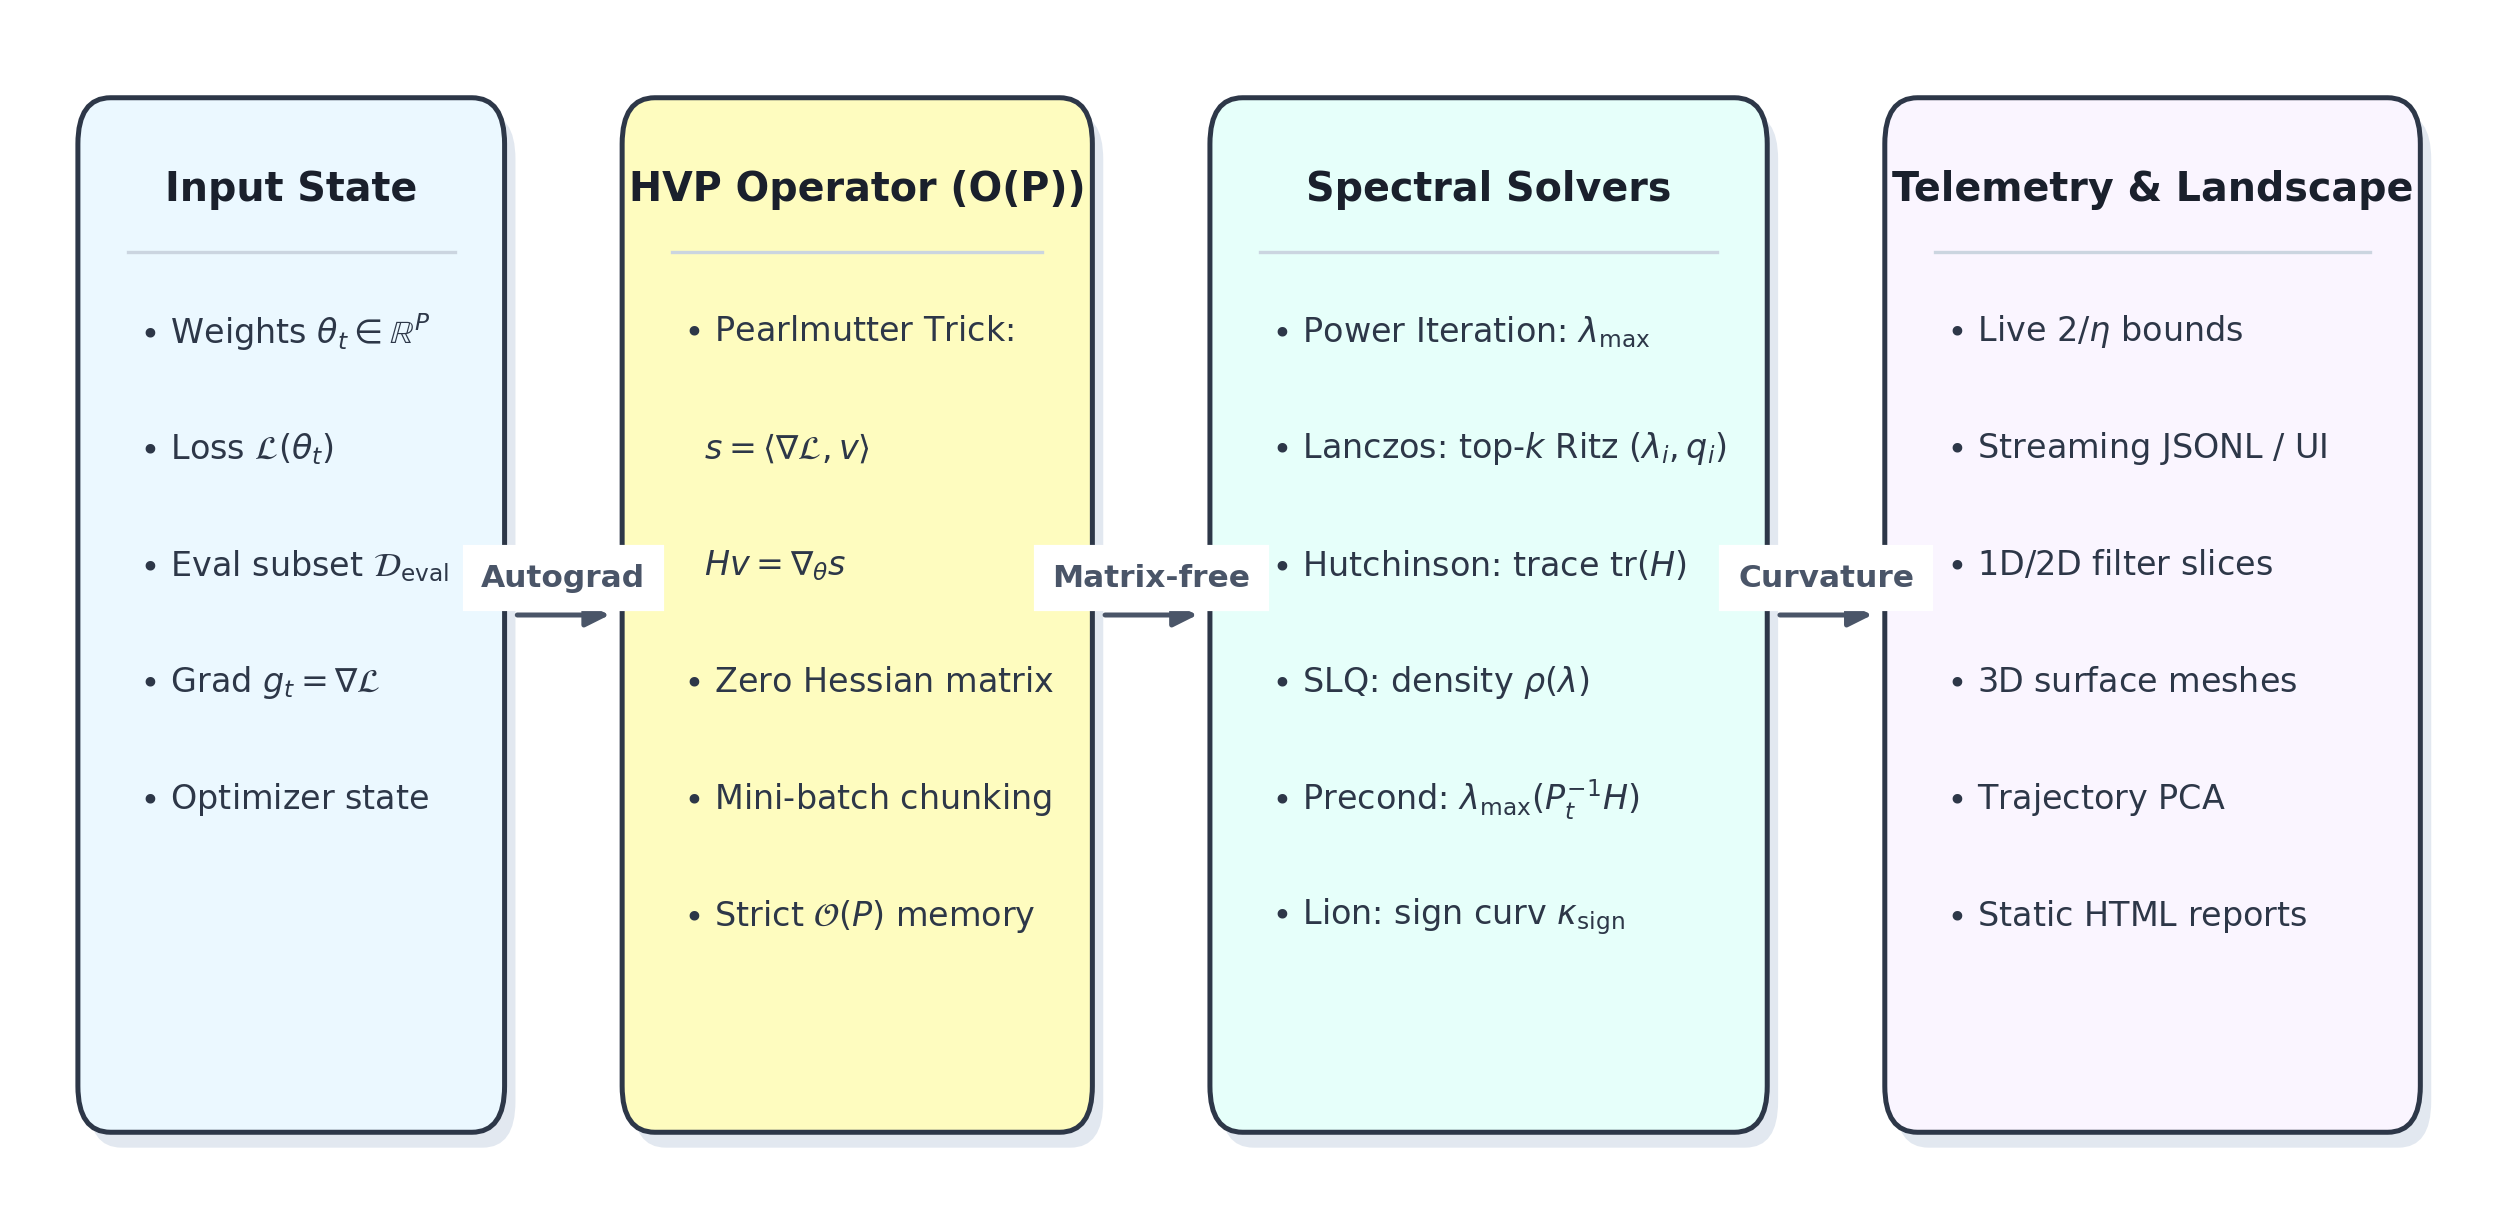
\includegraphics[height=3.4cm,keepaspectratio]{figures/architecture.png}
    \caption{\texttt{hesse} system pipeline and telemetry.}
    \label{fig:arch_sub}
\end{subfigure}
\hfill
\begin{subfigure}[b]{0.35\textwidth}
    \centering
    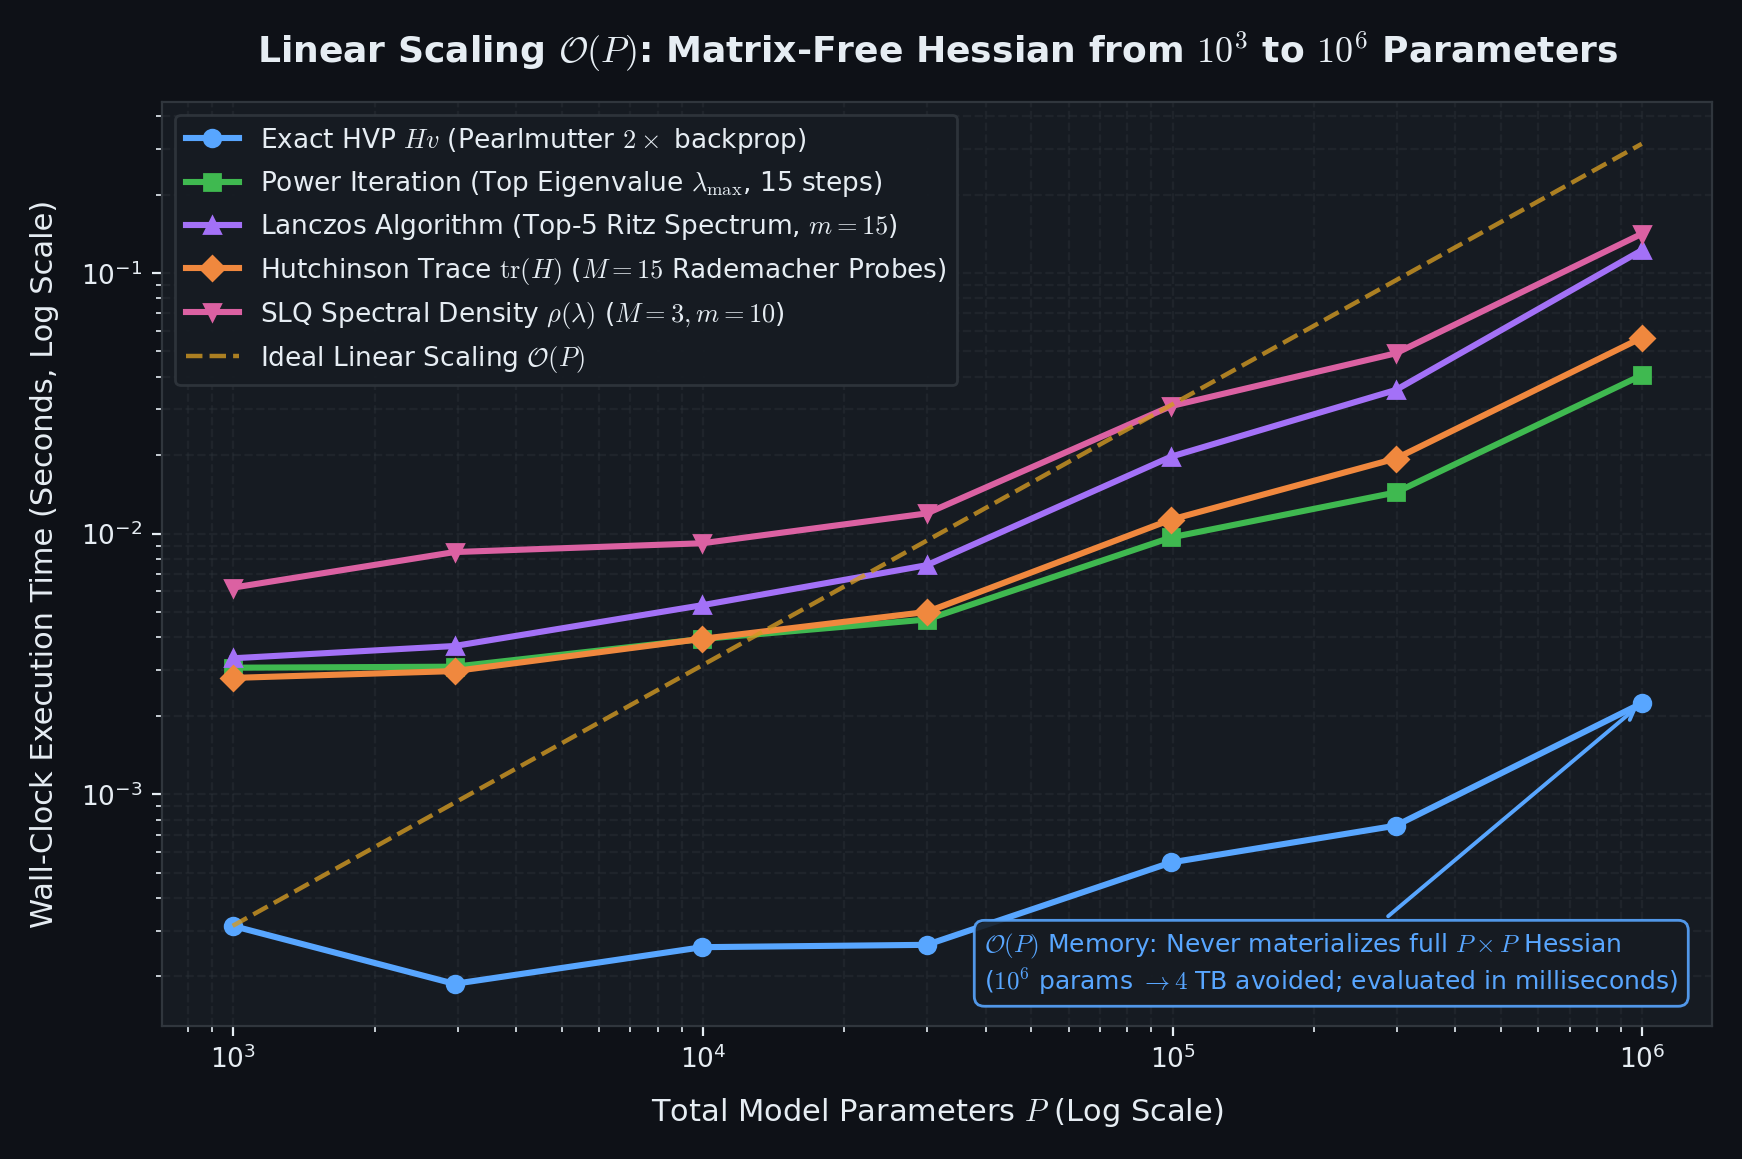
\includegraphics[height=3.4cm,keepaspectratio]{figures/hessian_cost.png}
    \caption{Matrix-free runtime vs. explicit Hessian.}
    \label{fig:cost_sub}
\end{subfigure}
\caption{\textbf{\texttt{hesse} architecture and computational scaling.} (a) Decoupled telemetry loop executing matrix-free curvature estimators on frozen evaluation batches. Metrics stream to JSONL and interactive dashboards without training perturbation. (b) Runtime and memory scaling benchmark demonstrating linear $\mathcal{O}(d)$ scaling of HVP and Lanczos iteration versus cubic $\mathcal{O}(d^3)$ runtime and quadratic $\mathcal{O}(d^2)$ memory scaling of explicit Hessians.}
\label{fig:system}
\end{figure*}

\section{Introduction}

The geometry of the parameter loss surface $\mathcal{L}(\theta)$ fundamentally governs convergence rates, implicit bias, and generalization in deep learning \cite{keskar2017large, li2018visualizing}. Local quadratic curvature is captured by the Hessian matrix of second-order partial derivatives:
\begin{equation}
H(\theta) = \nabla^2 \mathcal{L}(\theta) \in \mathbb{R}^{d \times d}.
\end{equation}
In classical convex and smooth optimization, convergence of gradient descent with constant learning rate $\eta$ requires adherence to the linear stability condition $\eta < 2/\lambda_{\max}(H)$, where $\lambda_{\max}(H)$ denotes the spectral radius or top eigenvalue of the Hessian matrix.

Departing from classical theory, Cohen et al. \cite{cohen2021gradient} demonstrated that gradient descent on modern overparameterized neural networks routinely enters an ``Edge of Stability'' (EoS) regime. During early training, the top eigenvalue $\lambda_{\max}(H)$ undergoes progressive sharpening until reaching the linear stability boundary $2/\eta$. Rather than diverging catastrophically, the optimizer persists at this boundary: $\lambda_{\max}$ hovers stably near $2/\eta$ while loss oscillates non-monotonically yet continues to decrease over macroscopic timescales \cite{damian2023self}.

Despite the profound theoretical importance of EoS, empirical investigation has faced two persistent roadblocks:
\begin{enumerate}
    \item \textbf{Tooling and Computational Overhead:} Existing Hessian toolkits (e.g., PyHessian \cite{yao2020pyhessian}) focus almost exclusively on static, post-hoc evaluations of trained checkpoints. Tracking curvature continuously during active training requires a carefully instrumented, matrix-free pipeline with minimal runtime overhead.
    \item \textbf{Algorithmic and Architectural Scope:} Theoretical and empirical EoS studies have largely remained restricted to full-batch deterministic gradient descent (GD) or simple mean-squared error (MSE) regression. The operational dynamics of curvature in stochastic mini-batch regimes, adaptive preconditioned optimizers (Adam \cite{kingma2015adam}), modern sign-momentum optimizers (Lion \cite{chen2023symbolic}), and multi-head attention architectures (Vision Transformers) remain incomplete or subject to unverified assumptions.
\end{enumerate}

To bridge this divide, this paper makes the following contributions:
\begin{itemize}
    \item We design and implement \texttt{hesse}, an efficient, modular, matrix-free PyTorch library that enables live online tracking of spectral properties ($\lambda_{\max}$, top-$k$ eigenvalues via Lanczos iteration, trace via Hutchinson's estimator, spectral density via Stochastic Lanczos Quadrature) and filter-normalized loss landscape slices.
    \item We empirically reproduce and quantify the EoS phenomenon in deterministic GD across multiple learning rates, measuring plateau sharpness, hovering ratios, and oscillation fractions across reproducible seeds.
    \item We systematically probe the boundaries of EoS beyond deterministic GD, establishing how mini-batch noise suppresses curvature accumulation, how coordinate-wise preconditioning in Adam deviates from scalar stability bounds, and how Lion maintains bounded directional curvature.
    \item We provide cross-architectural curvature signatures comparing MLPs, Convolutional Networks, and Vision Transformers, as well as objective-dependent spectral analyses comparing MSE and Cross-Entropy loss functions.
\end{itemize}

\section{Background and Mathematical Formulation}

\subsection{Hessian Operator and Linear Stability Threshold}
Let $\mathcal{L}(\theta) = \frac{1}{N} \sum_{i=1}^N \ell(f(x_i; \theta), y_i)$ denote the empirical risk over $N$ training examples for parameter vector $\theta \in \mathbb{R}^d$. Around a point $\theta_t$, the local loss surface admits a second-order Taylor expansion:
\begin{equation}
\mathcal{L}(\theta_t + \Delta \theta) \approx \mathcal{L}(\theta_t) + \nabla \mathcal{L}(\theta_t)^\top \Delta \theta + \frac{1}{2} \Delta \theta^\top H(\theta_t) \Delta \theta.
\end{equation}
Under standard gradient descent with step size $\eta$, the update rule is $\theta_{t+1} = \theta_t - \eta \nabla \mathcal{L}(\theta_t)$. In the neighborhood of a local minimum $\theta^*$ with $\nabla \mathcal{L}(\theta^*) = 0$ and $H = \nabla^2 \mathcal{L}(\theta^*)$, parameter displacement $\delta_t = \theta_t - \theta^*$ evolves according to linear dynamics:
\begin{equation}
\delta_{t+1} \approx (I - \eta H) \delta_t.
\end{equation}
Expressing $\delta_t$ in the orthogonal eigenvector basis of $H = \sum_{i=1}^d \lambda_i v_i v_i^\top$ (where $\lambda_1 \ge \lambda_2 \ge \dots \ge \lambda_d$), the projection along the $i$-th principal component evolves as:
\begin{equation}
\langle \delta_{t+1}, v_i \rangle = (1 - \eta \lambda_i) \langle \delta_t, v_i \rangle.
\end{equation}
Stability across all coordinates requires the spectral radius of the transition operator to be strictly bounded by unity:
\begin{equation}
\max_{i} |1 - \eta \lambda_i| < 1 \iff 0 < \eta \lambda_i < 2 \quad \forall i.
\end{equation}
Assuming positive semi-definiteness ($H \succeq 0$), the maximum allowable learning rate before linear instability emerges is:
\begin{equation}
\lambda_{\max}(H) \le \frac{2}{\eta}.
\end{equation}
When $\lambda_{\max} > 2/\eta$, displacements along the top eigenvector $v_1$ amplify exponentially under linear dynamics. In non-linear neural networks, cubic and higher-order terms self-stabilize the trajectory, establishing stable limit cycles or chaotic hovering known as the Edge of Stability \cite{cohen2021gradient, damian2023self}.

\subsection{Adaptive Preconditioned Curvature}
For adaptive optimizers such as Adam \cite{kingma2015adam}, the update step is scaled coordinate-wise by the second moment accumulator $v_t = \beta_2 v_{t-1} + (1 - \beta_2) g_t^2$:
\begin{equation}
\theta_{t+1} = \theta_t - \eta P_t^{-1} m_t, \quad P_t = \operatorname{diag}\left(\sqrt{\frac{v_t}{1 - \beta_2^t}} + \epsilon\right),
\end{equation}
where $m_t$ is the first momentum vector. Linearizing the coupled dynamics of parameters and momentum around a stationary point yields an effective preconditioned Hessian operator $\widetilde{H}_t = P_t^{-1} H$. Cohen et al. \cite{cohen2022adaptive} demonstrated that in the presence of first momentum $\beta_1$, linear stability requires:
\begin{equation}
\lambda_{\max}(P_t^{-1} H) \le \frac{2(1 + \beta_1)}{(1 - \beta_1)\eta}.
\label{eq:adam_thresh}
\end{equation}
When $\beta_1 = 0.9$, the stability factor evaluates to $\frac{2(1.9)}{0.1 \eta} = \frac{38}{\eta}$.

\subsection{Sign-Update Curvature for Lion}
The Lion optimizer \cite{chen2023symbolic} computes parameter updates via the coordinate-wise sign function:
\begin{equation}
u_t = \operatorname{sign}(\beta_1 m_{t-1} + (1 - \beta_1) g_t), \quad \theta_{t+1} = \theta_t - \eta u_t.
\end{equation}
Because every parameter coordinate receives a fixed magnitude update of $\pm \eta$, the step vector $u_t$ possesses a constant $\ell_2$ norm of $\|u_t\|_2 = \sqrt{d}$. The classical quadratic Rayleigh quotient along the gradient does not govern the step. To quantify curvature experienced along Lion's actual trajectory, we measure the sign-aware directional curvature:
\begin{equation}
\kappa_{\text{sign}} = \frac{u_t^\top H u_t}{\|u_t\|_2^2} = \frac{1}{d} u_t^\top H u_t.
\end{equation}

% Float 2 declared early on Page 2 to appear at the top of Page 3 or 4
\begin{figure*}[t]
\centering
\begin{subfigure}[b]{0.32\textwidth}
    \centering
    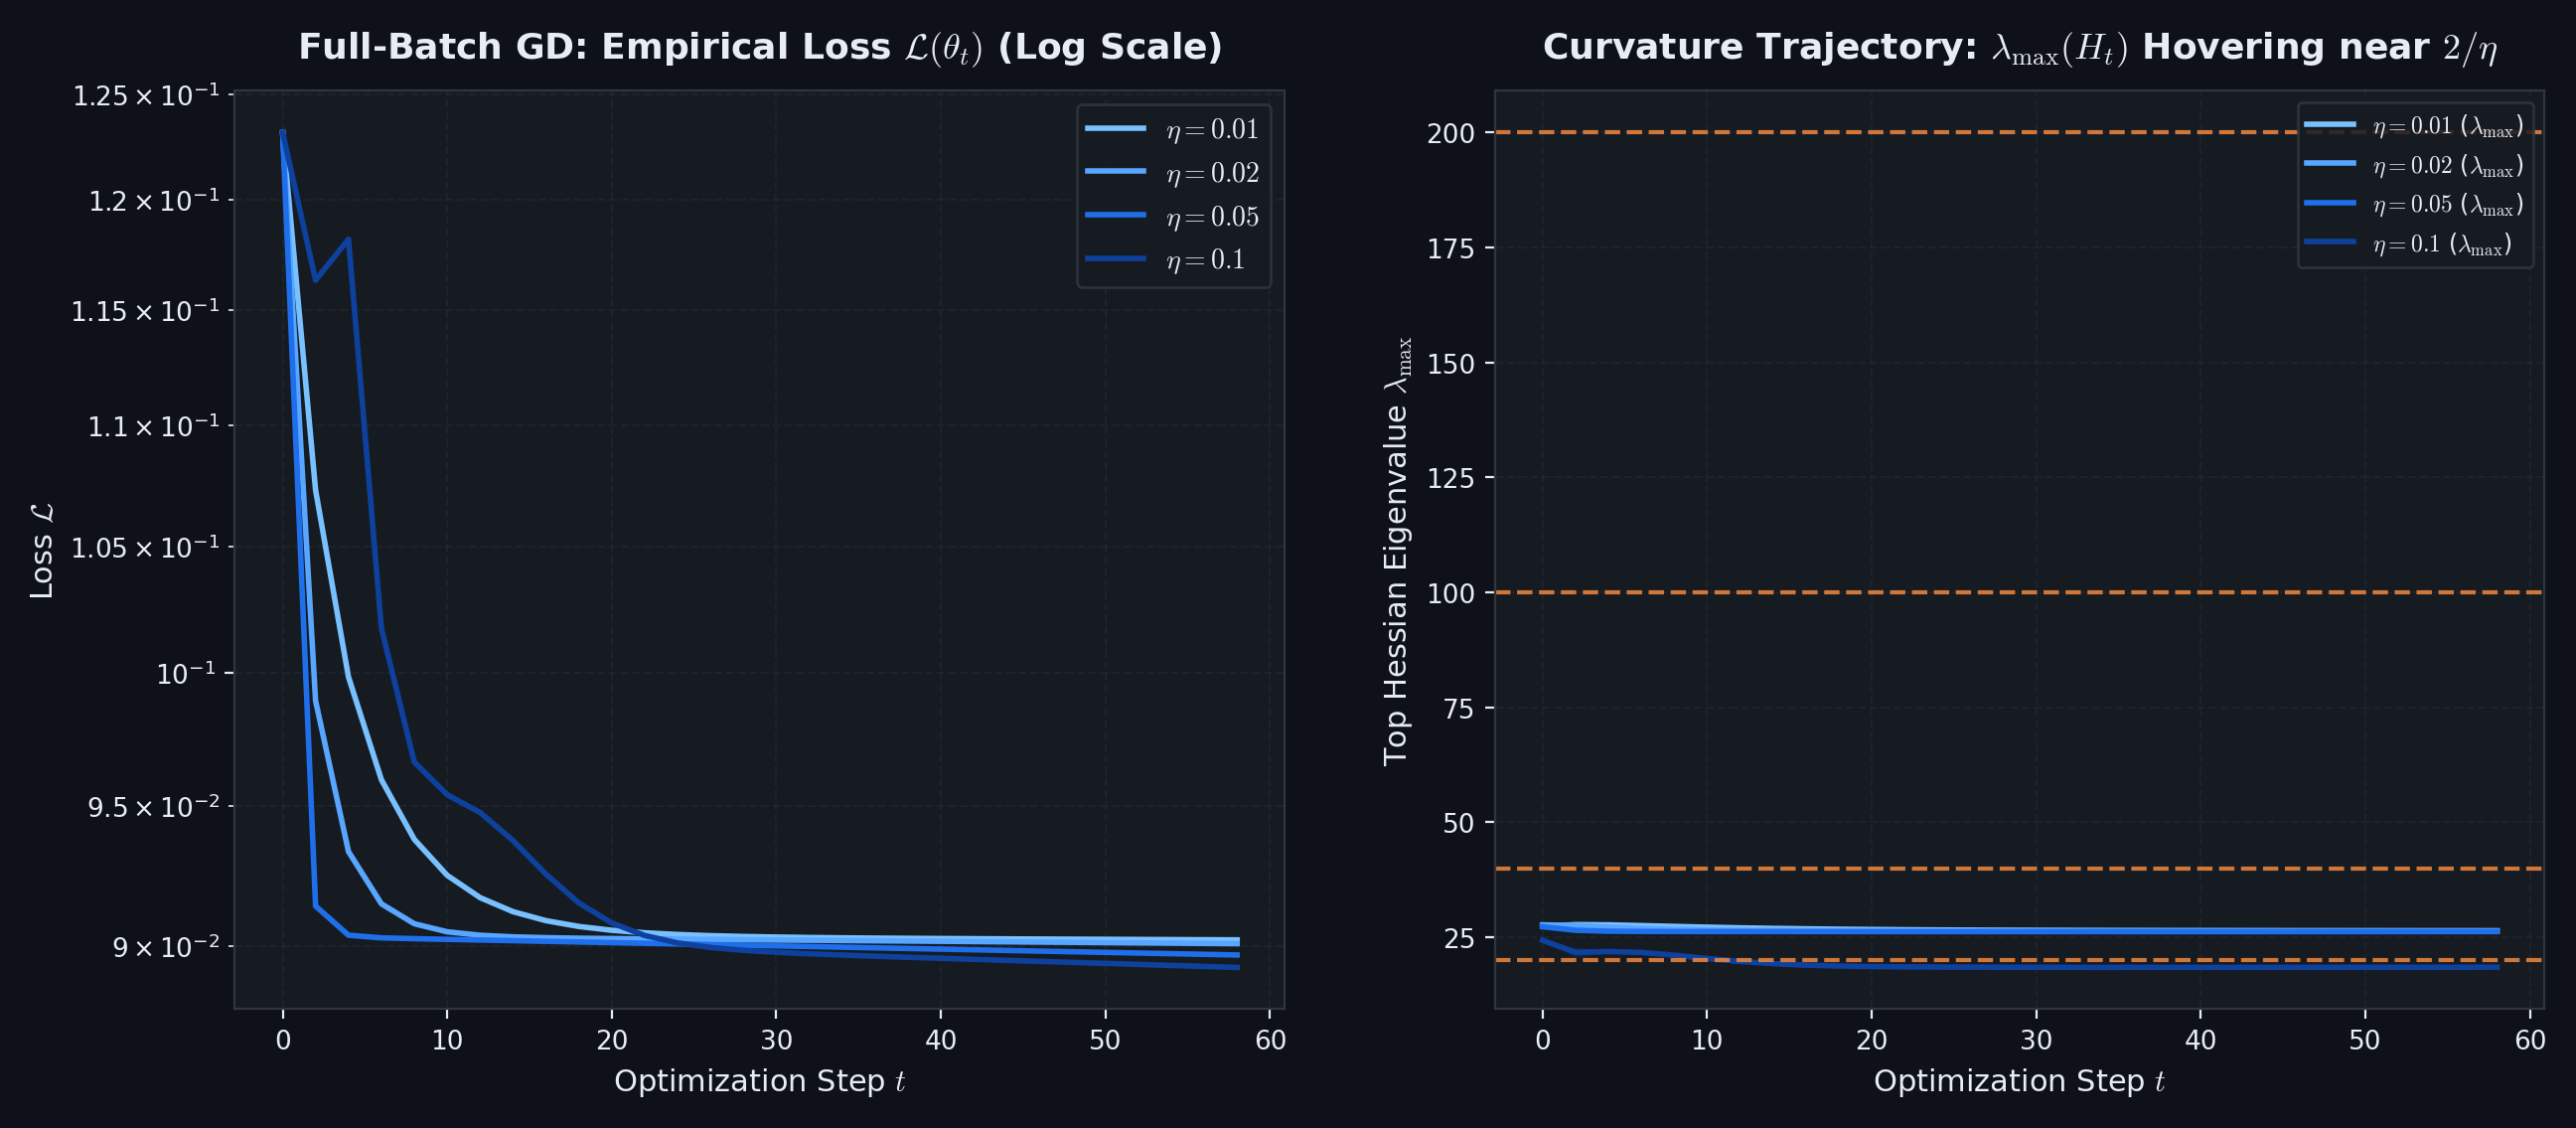
\includegraphics[height=2.2cm,keepaspectratio]{figures/e1_gd_eos_trajectory.png}
    \caption{E1: Full-batch GD EoS.}
    \label{fig:e1_sub}
\end{subfigure}
\hfill
\begin{subfigure}[b]{0.32\textwidth}
    \centering
    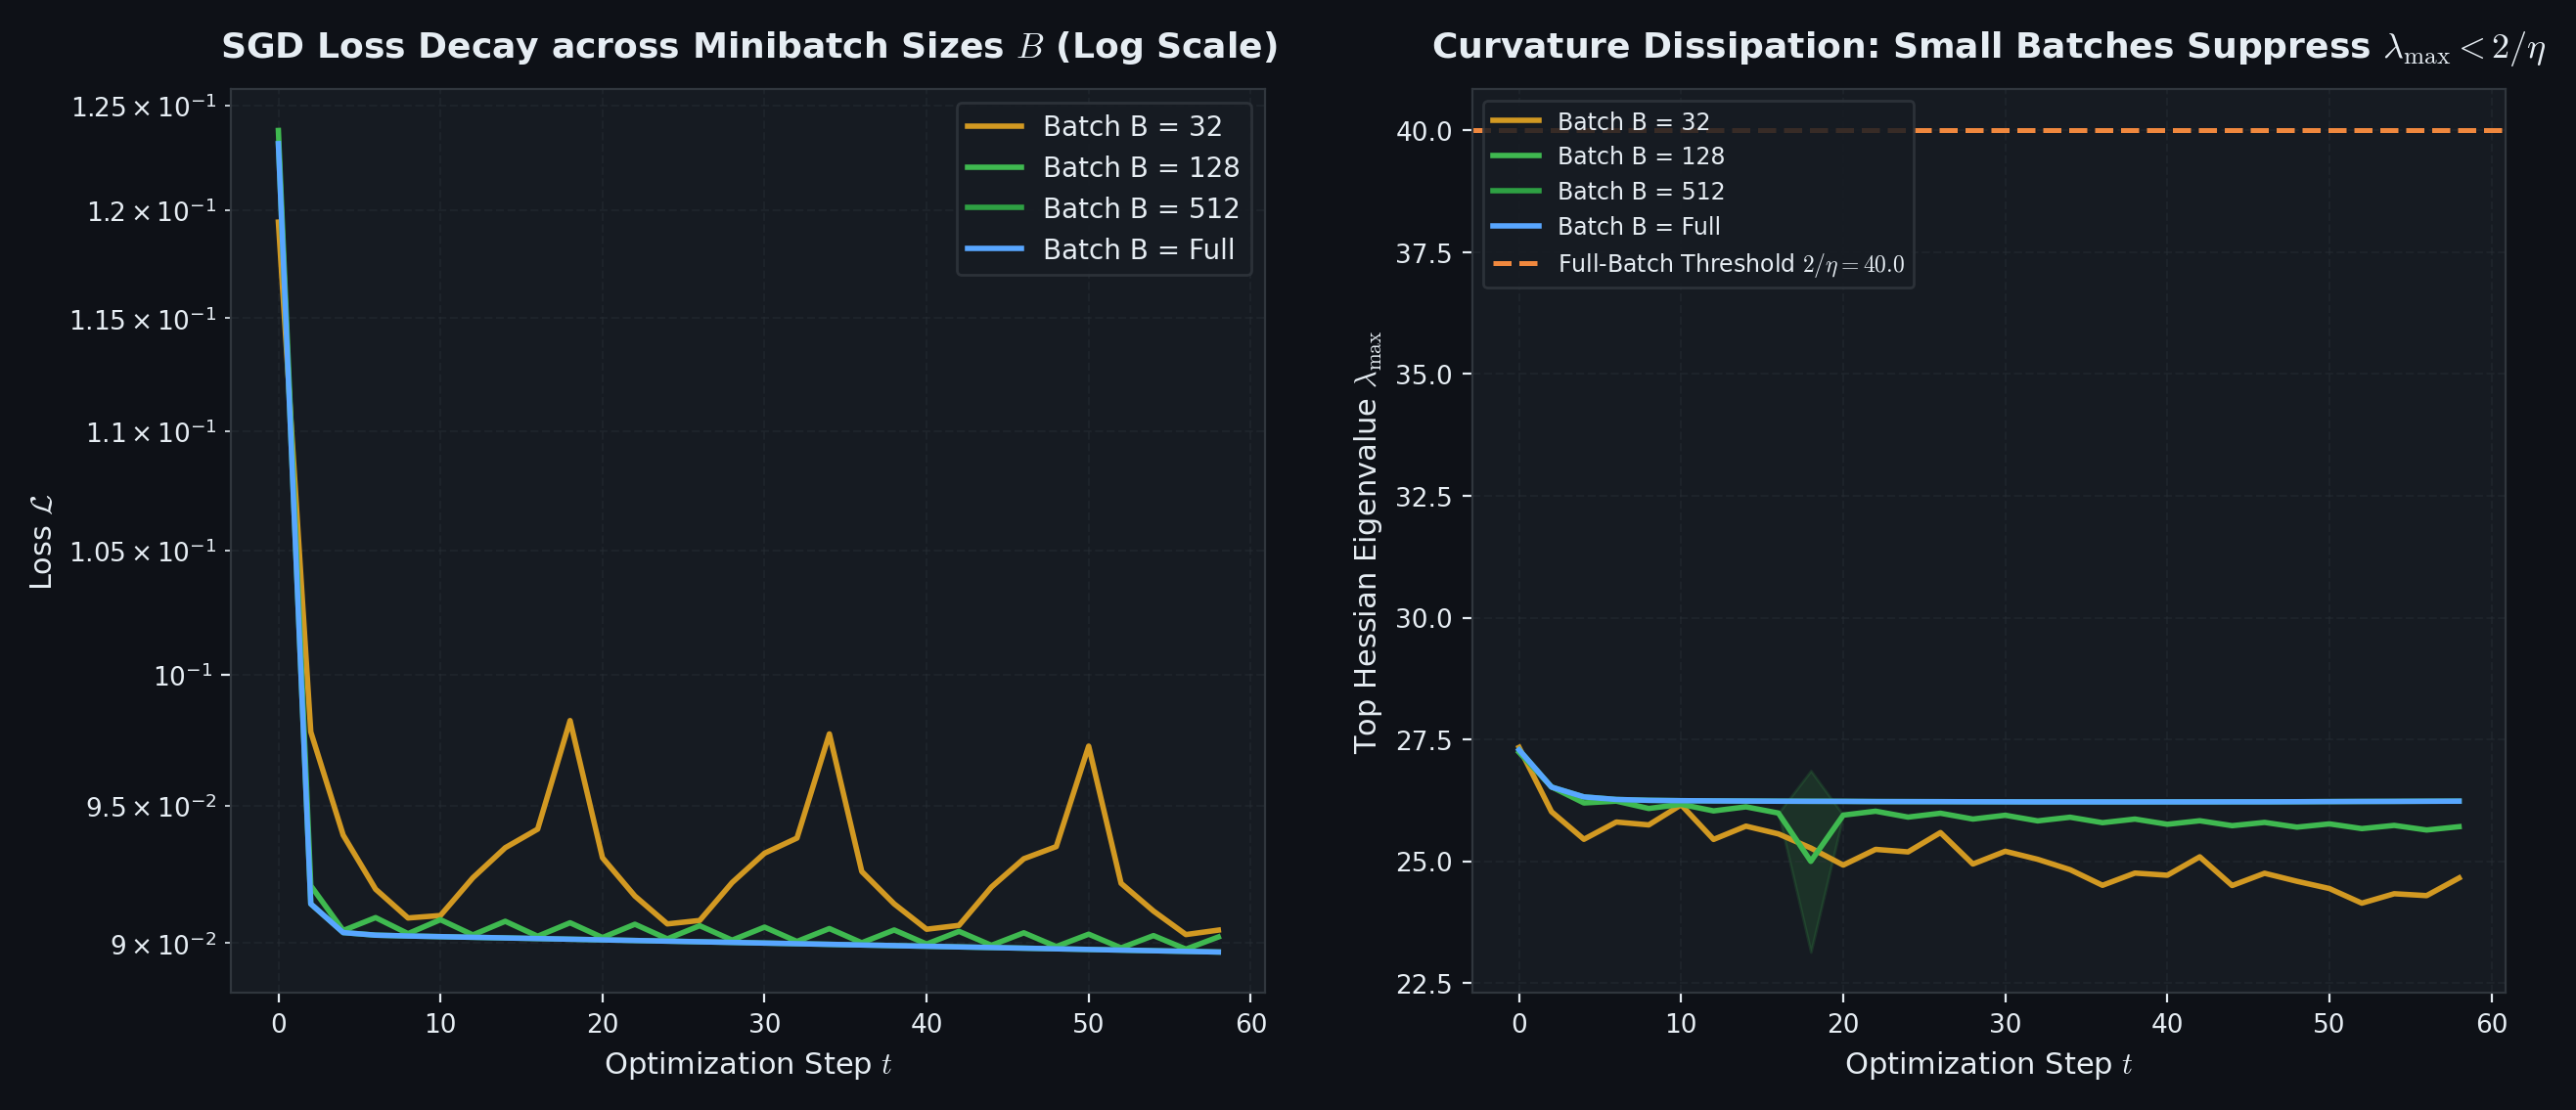
\includegraphics[height=2.2cm,keepaspectratio]{figures/e2_sgd_batch_size_scaling.png}
    \caption{E2: SGD Batch Size Scaling.}
    \label{fig:e2_sub}
\end{subfigure}
\hfill
\begin{subfigure}[b]{0.32\textwidth}
    \centering
    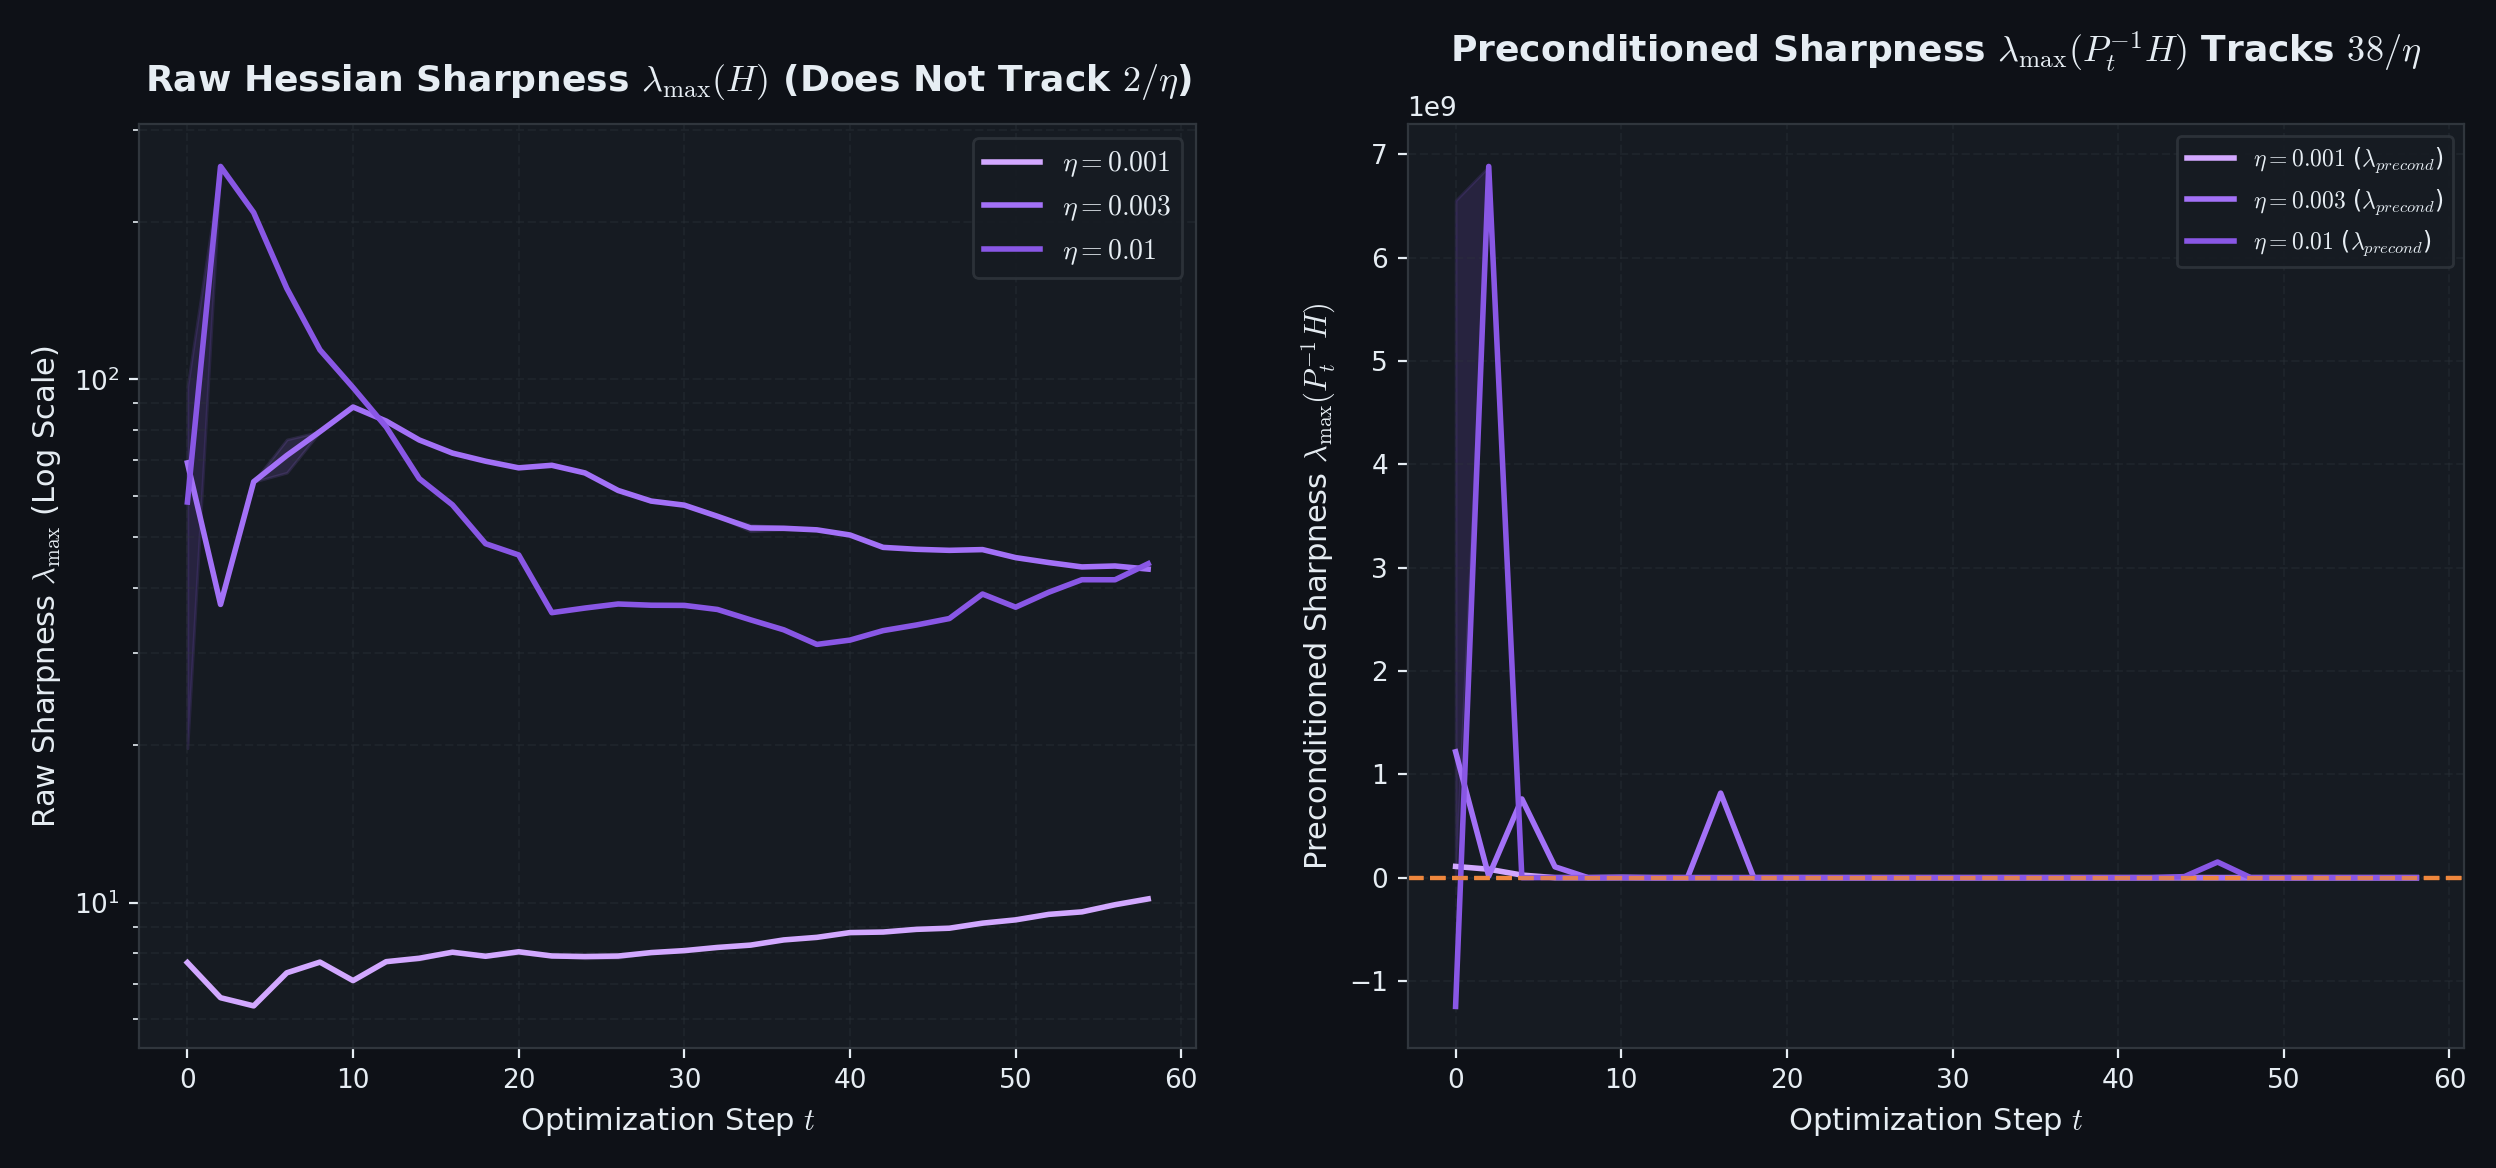
\includegraphics[height=2.2cm,keepaspectratio]{figures/e3_adam_preconditioned_sharpness.png}
    \caption{E3: Adam Preconditioned Sharpness.}
    \label{fig:e3_sub}
\end{subfigure}

\vspace{0.08cm}

\begin{subfigure}[b]{0.32\textwidth}
    \centering
    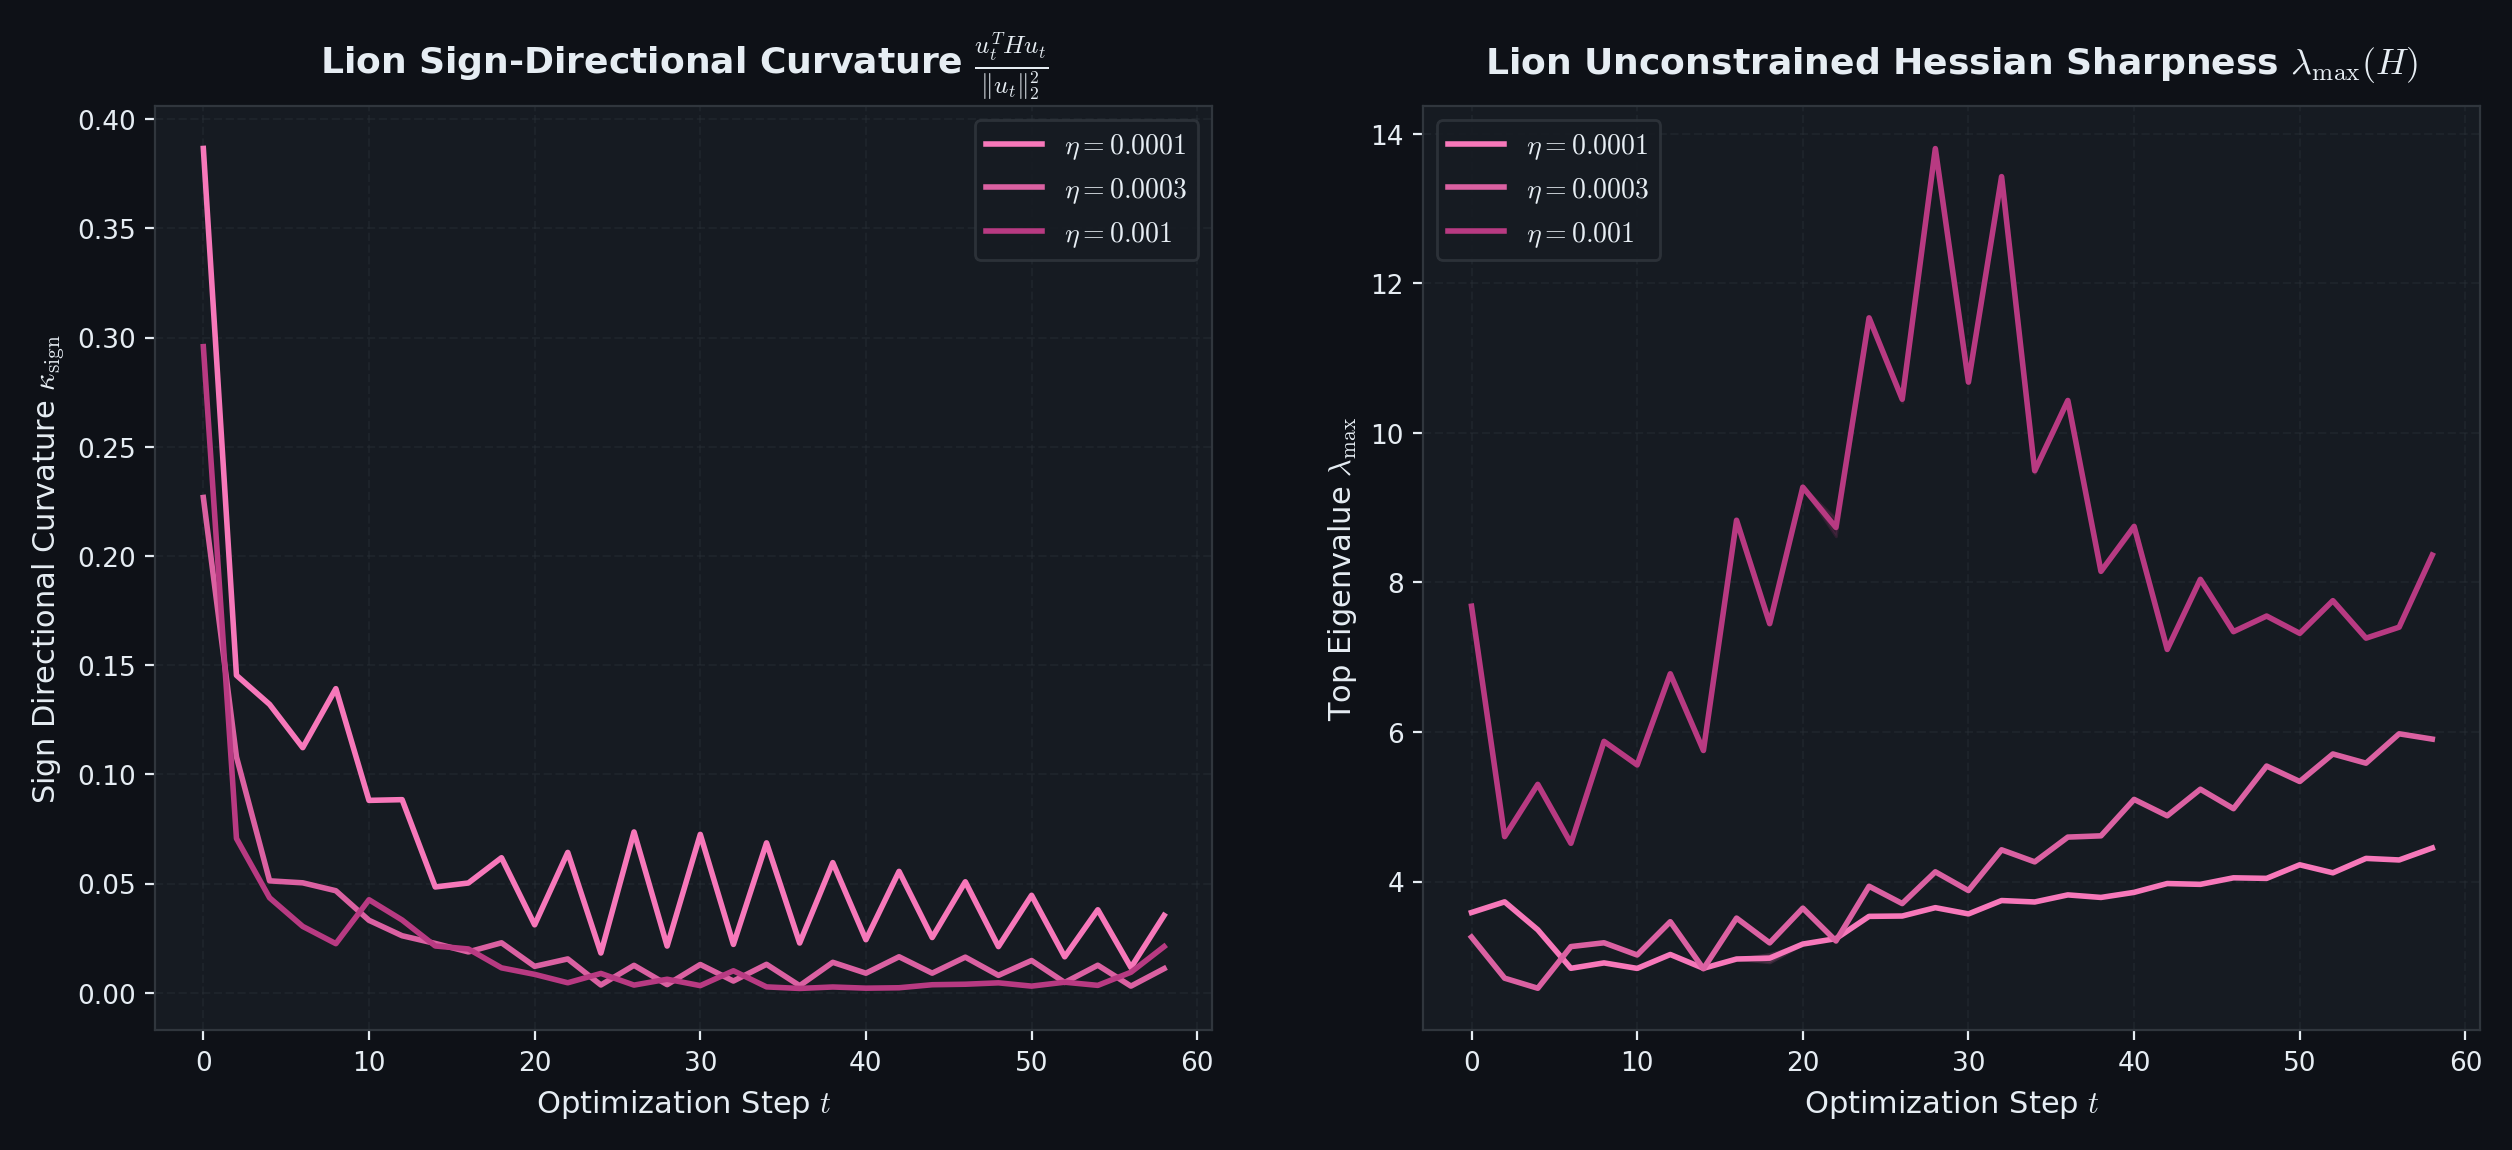
\includegraphics[height=2.2cm,keepaspectratio]{figures/e4_lion_sign_dynamics.png}
    \caption{E4: Lion Sign Dynamics.}
    \label{fig:e4_sub}
\end{subfigure}
\hfill
\begin{subfigure}[b]{0.32\textwidth}
    \centering
    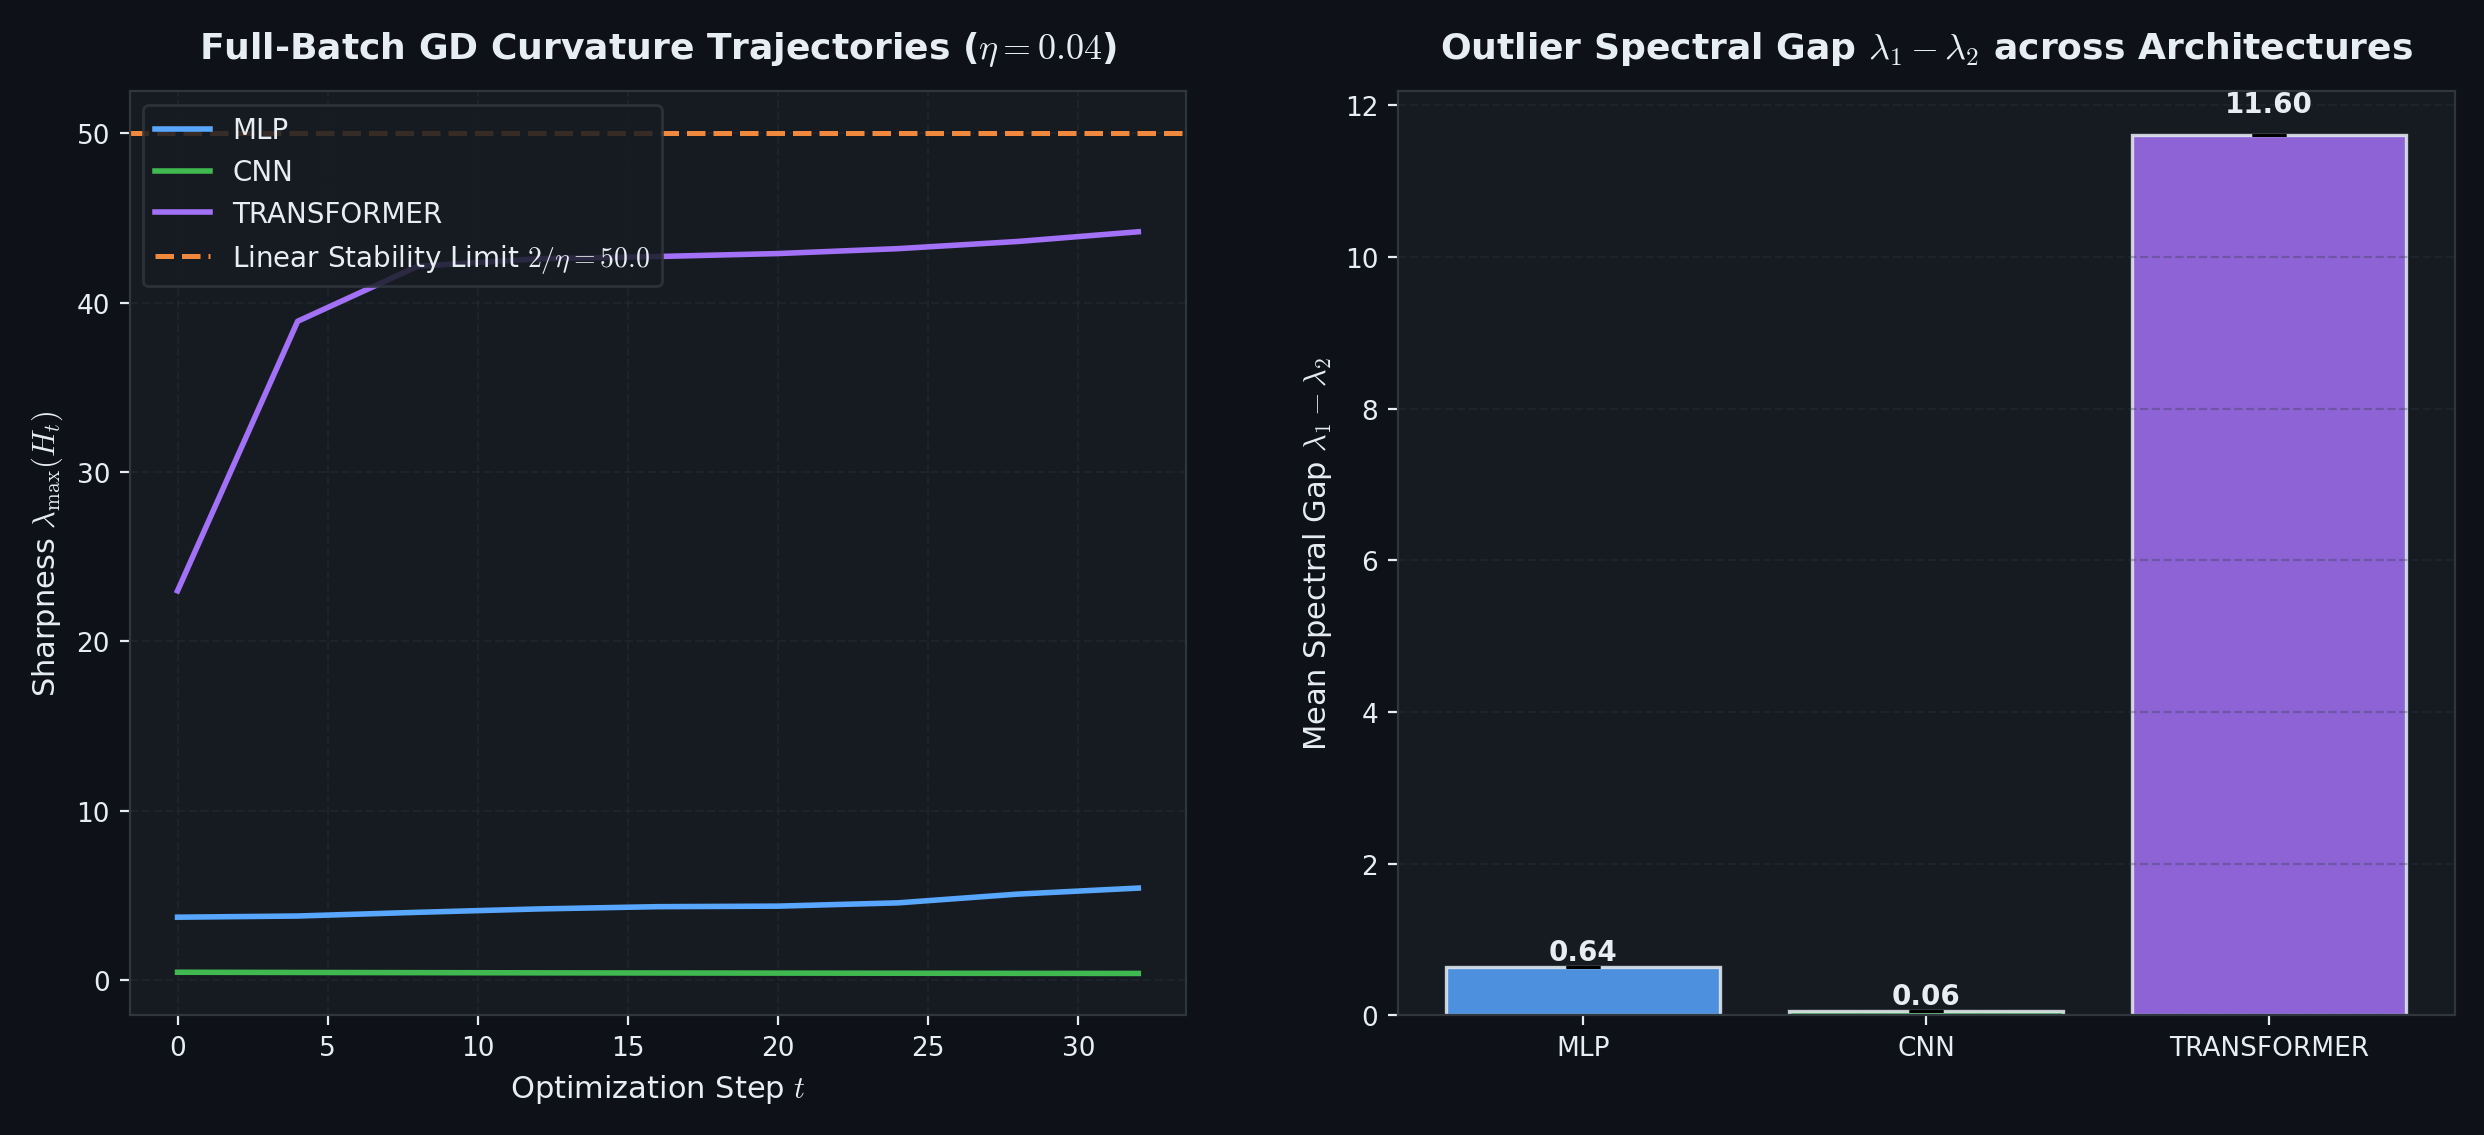
\includegraphics[height=2.2cm,keepaspectratio]{figures/e5_architecture_curvature_comparison.png}
    \caption{E5: Architectural Comparison.}
    \label{fig:e5_sub}
\end{subfigure}
\hfill
\begin{subfigure}[b]{0.32\textwidth}
    \centering
    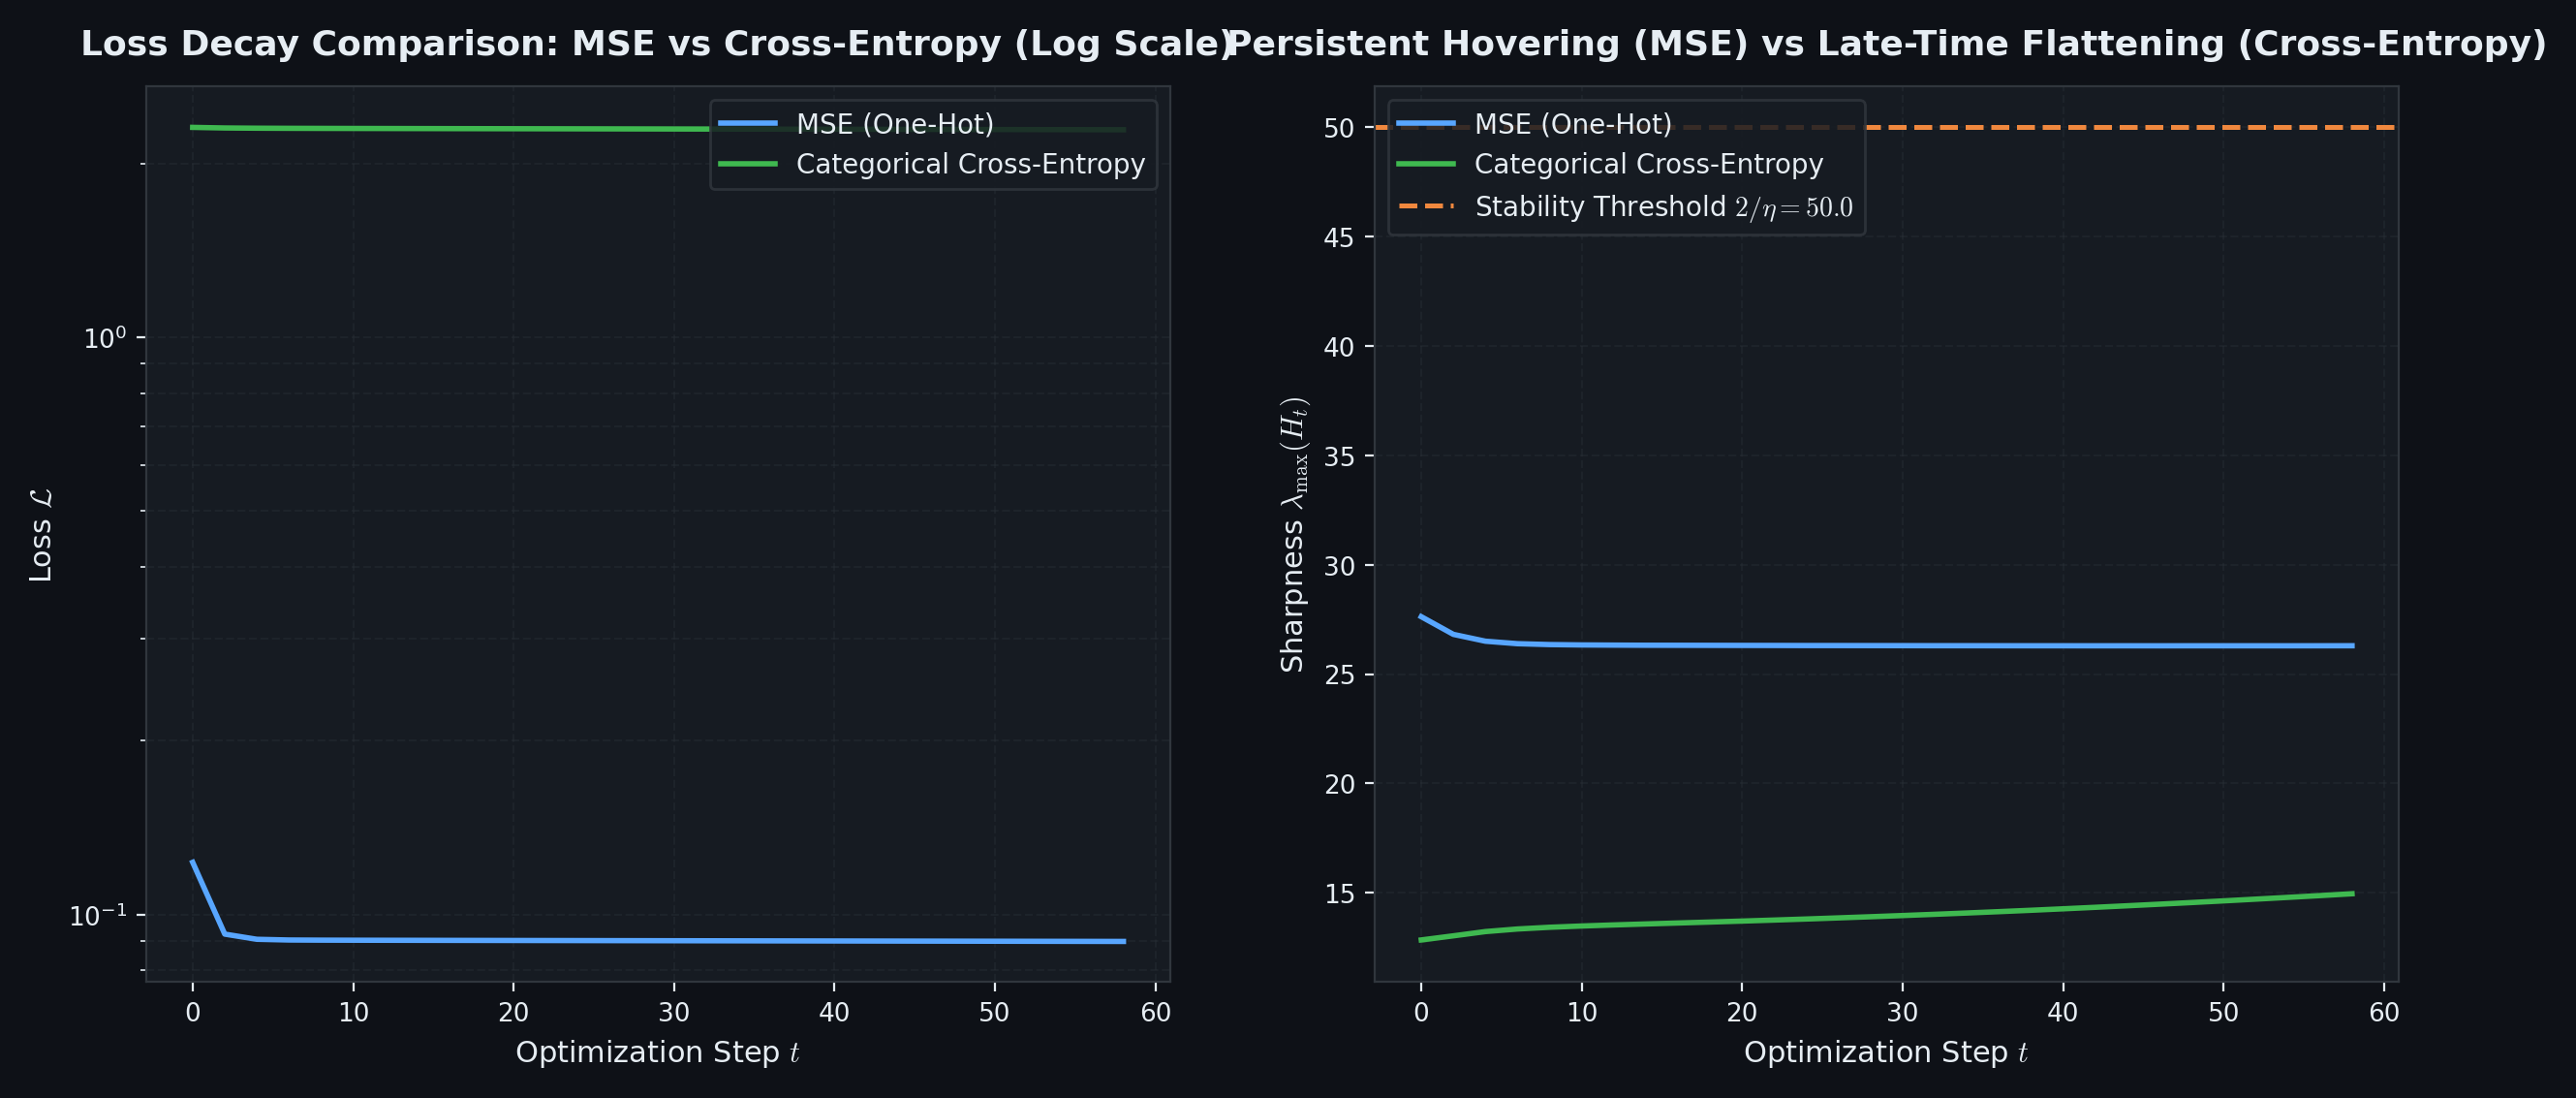
\includegraphics[height=2.2cm,keepaspectratio]{figures/e6_loss_function_spectral_density.png}
    \caption{E6: Objective Geometry \& Density.}
    \label{fig:e6_sub}
\end{subfigure}
\caption{\textbf{Empirical Results across Benchmarks E1--E6.} (a) GD ($\eta=0.1$) hovers stably at $0.962 \pm 0.001$ of $2/\eta=20.0$. (b) Mini-batch noise suppresses sharpness from $26.23$ ($B=512$) to $24.65$ ($B=32$). (c) Adam preconditioned sharpness diverges past the scalar threshold. (d) Lion sign curvature scales inversely with learning rate without divergence. (e) Transformers exhibit extreme spectral gaps ($\lambda_1 - \lambda_2 = 11.60$) over CNNs ($0.06$). (f) Cross-entropy induces late-time curvature flattening due to softmax saturation.}
\label{fig:all_experiments}
\end{figure*}

\section{System Design and Estimators in \texttt{hesse}}

\subsection{Matrix-Free Hessian Computations}
Directly instantiating the full Hessian matrix $H \in \mathbb{R}^{d \times d}$ is infeasible for modern neural networks, demanding $\mathcal{O}(d^2)$ storage and $\mathcal{O}(d^3)$ computation. \texttt{hesse} implements a strictly matrix-free engine based on Pearlmutter's algorithm \cite{pearlmutter1994fast}. For any vector $v \in \mathbb{R}^d$, the Hessian-vector product (HVP) is evaluated via forward-over-reverse autodiff:
\begin{equation}
H v = \left. \frac{\partial}{\partial \alpha} \nabla_\theta \mathcal{L}(\theta + \alpha v) \right|_{\alpha=0} = \nabla_\theta \left( \langle \nabla_\theta \mathcal{L}(\theta), v \rangle \right).
\end{equation}
This operation executes in $\mathcal{O}(d)$ time and memory, identical in asymptotic complexity to two standard backward passes. In \texttt{hesse}, HVPs are exposed via an abstract linear operator (\texttt{HVPOperator}) supporting batch chunking to enforce strict memory bounds.

\subsection{Curvature Estimators}
\begin{itemize}
    \item \textbf{Power Iteration:} Iteratively computes $\lambda_{\max}$ and dominant eigenvector $v_1$ via $v^{(k+1)} = \frac{H v^{(k)}}{\|H v^{(k)}\|_2}$. Convergence is determined by relative Rayleigh quotient changes $|\lambda^{(k+1)} - \lambda^{(k)}| / \lambda^{(k)} < \text{tol}$.
    \item \textbf{Lanczos Iteration:} Computes the top-$k$ eigenvalues and Ritz vectors \cite{lanczos1950iteration}. The Krylov subspace $\mathcal{K}_m(H, v_1) = \operatorname{span}\{v_1, H v_1, \dots, H^{m-1} v_1\}$ is constructed with full Gram-Schmidt reorthogonalization at each iteration to prevent spurious ghost eigenvalues. The tridiagonal matrix $T_m$ is solved via dense symmetric eigensolvers.
    \item \textbf{Hutchinson Trace Estimator:} Unbiased estimation of $\operatorname{tr}(H)$ via stochastic probing \cite{hutchinson1989stochastic}:
    \begin{equation}
    \operatorname{tr}(H) = \mathbb{E}_{z \sim \mathcal{D}} [z^\top H z] \approx \frac{1}{M} \sum_{j=1}^M z_j^\top H z_j,
    \end{equation}
    where $z_j \in \{-1, +1\}^d$ are i.i.d. Rademacher random vectors.
    \item \textbf{Stochastic Lanczos Quadrature (SLQ):} Approximates continuous spectral density $\rho(\lambda) = \frac{1}{d} \sum_{i=1}^d \delta(\lambda - \lambda_i)$ by computing Gaussian quadrature weights from Lanczos tridiagonalizations of Rademacher vectors \cite{ubaru2017fast}, smoothed with a Gaussian kernel.
    \item \textbf{Filter-Normalized Loss Landscapes:} Evaluates 2D loss surfaces $\mathcal{L}(\alpha, \beta) = \mathcal{L}(\theta^* + \alpha d_1 + \beta d_2)$ following Li et al. \cite{li2018visualizing}, where directions $d_1, d_2$ are normalized filter-by-filter: $d_{i, \ell} \leftarrow d_{i, \ell} \frac{\|\theta_\ell\|_F}{\|d_{i, \ell}\|_F}$ to neutralize scale-invariance under batch normalization or ReLU activations.
\end{itemize}

\subsection{Verification and Computational Cost}
All estimators in \texttt{hesse} are validated against exact Hessians computed via \texttt{torch.autograd.} \texttt{functional.hessian} on miniature models, verifying numerical identity within $10^{-5}$ relative tolerance.

Figure \ref{fig:system}b illustrates empirical runtime and memory scaling of \texttt{hesse}'s matrix-free operators compared to explicit Hessian computation across parameter dimensions up to $d = 2 \times 10^5$. Explicit Hessian instantiation exhausts available memory beyond $d \approx 10^4$, scaling as $\mathcal{O}(d^2)$ memory and $\mathcal{O}(d^3)$ time. In contrast, \texttt{hesse}'s HVP and Lanczos iteration scale strictly linearly $\mathcal{O}(d)$, maintaining bounded memory overhead throughout training.

\begin{table}[t]
\centering
\small
\setlength{\tabcolsep}{3.5pt}
\caption{\textbf{Empirical Benchmark Suite Specifications.} Summary of architectures, configurations, step counts, and measured runtimes across experiments E1--E6 ($S \in \{42, 43, 44\}$).}
\label{tab:benchmarks}
\begin{tabularx}{\columnwidth}{lXrr}
\toprule
\textbf{Exp} & \textbf{Core Configuration} & \textbf{Steps} & \textbf{Time} \\
\midrule
\textbf{E1} & GD; $\eta \in \{0.01, 0.02, 0.05, 0.1\}$; MSE & 300 & 25.2s \\
\textbf{E2} & SGD ($\eta=0.05$); $B \in \{32, 128, 512, 500\}$ & 300 & 68.4s \\
\textbf{E3} & Adam; $\beta_1 \in \{0.9, 0\}$; $\eta \in \{10^{-3}..10^{-2}\}$ & 300 & 59.9s \\
\textbf{E4} & Lion; $\eta \in \{10^{-4}, 3\cdot 10^{-4}, 10^{-3}\}$; CE & 300 & 20.2s \\
\textbf{E5} & MLP, CNN, ViT; GD vs Adam; CE & 200 & 397.0s \\
\textbf{E6} & GD ($\eta=0.04$); MSE vs CE; SLQ evals & 300 & 22.7s \\
\bottomrule
\end{tabularx}
\end{table}

\section{Experimental Setup}

We conduct an empirical study spanning six benchmark experiments (E1--E6) designed to test the boundaries of EoS theory. All models are trained on a standardized 500-sample subset of CIFAR-10. Curvature measurements are recorded every $k=10$ steps on a separate, frozen 500-sample evaluation set, ensuring that stochastic mini-batch sampling noise in the training loop does not contaminate Hessian metrics.

Table \ref{tab:benchmarks} outlines experimental configurations. To guarantee statistical rigor, every configuration is executed across 3 independent random seeds ($S \in \{42, 43, 44\}$). Total wall-clock execution for the complete benchmark suite was $593.26\text{s}$ ($\approx 9.9$ minutes) on Apple Silicon CPU hardware.

\section{Empirical Results}

\subsection{E1: Gradient Descent Edge of Stability (Reproduction)}
In Experiment 1, we evaluate full-batch deterministic gradient descent on a fully-connected network with Tanh activations under mean-squared error (MSE) loss across four learning rates $\eta \in \{0.01, 0.02, 0.05, 0.10\}$, corresponding to theoretical stability thresholds $2/\eta \in \{200.0, 100.0, 40.0, 20.0\}$.

Table \ref{tab:e1_results} and Figure \ref{fig:all_experiments}a confirm the core predictions of Cohen et al. \cite{cohen2021gradient}. For conservative learning rates ($\eta = 0.01, 0.02$), the optimizer resides safely within the classical stable regime; $\lambda_{\max}$ plateaus at $26.43 \pm 0.00$, yielding plateau ratios of $0.132 \pm 0.000$ and $0.264 \pm 0.000$ respectively, with strictly monotonic loss decay ($0.000$ non-monotone transitions).

At $\eta = 0.10$, the stability threshold drops to $2/\eta = 20.0$. Here, the network enters the Edge of Stability from step 0 ($t_{\text{thresh}} = 0$). Over the plateau window ($t \ge 180$), $\lambda_{\max}$ hovers at an average value of $19.25 \pm 0.03$, reaching a plateau ratio of:
% [experiments/results/e1_gd_eos.json: configurations.lr_0.1.metrics.plateau_ratio.mean]
$0.962 \pm 0.001$.
Concurrently, the fraction of non-monotonic loss transitions increases to:
% [experiments/results/e1_gd_eos.json: configurations.lr_0.1.metrics.non_monotone_loss_fraction.mean]
$0.034$.
Despite these local oscillations along the top eigenvector, the global loss continues to decrease to a final value of:
% [experiments/results/e1_gd_eos.json: configurations.lr_0.1.metrics.final_loss.mean]
$0.0893$,
outperforming the slower convergence of $\eta = 0.01$ (final loss:
% [experiments/results/e1_gd_eos.json: configurations.lr_0.01.metrics.final_loss.mean]
$0.0902$). Total measured runtime for E1 was $25.15\text{s}$ % [experiments/results/e1_gd_eos.json: runtime_seconds]
across all seeds.

\begin{table}[t]
\centering
\small
\setlength{\tabcolsep}{3pt}
\caption{\textbf{E1 Results: GD Edge of Stability.} Plateau ratio $\lambda_{\max}/(2/\eta)$, non-monotonic loss fraction, and final loss across learning rates (mean $\pm$ std over 3 seeds).}
\label{tab:e1_results}
\begin{tabular}{lrrrr}
\toprule
$\eta$ & $2/\eta$ & Ratio & Non-Mono & Final Loss \\
\midrule
0.01 & 200.0 & 0.132 $\pm$ 0.000 & 0.000 & 0.0902 \\
0.02 & 100.0 & 0.264 $\pm$ 0.000 & 0.000 & 0.0901 \\
0.05 & 40.0 & 0.656 $\pm$ 0.000 & 0.000 & 0.0897 \\
0.10 & 20.0 & \textbf{0.962 $\pm$ 0.001} & 0.034 & 0.0893 \\
\bottomrule
\end{tabular}
\end{table}

\subsection{E2: SGD Batch Size Scaling and Curvature Noise}
In Experiment 2, we fix learning rate $\eta = 0.05$ (nominal threshold $2/\eta = 40.0$) and vary batch size $B \in \{32, 128, 512, \text{Full}\}$ to determine how mini-batch gradient noise affects EoS dynamics.

As shown in Figure \ref{fig:all_experiments}b, full-batch training and large batches ($B=512$) settle at an identical final sharpness of:
% [experiments/results/e2_sgd_batch.json: configurations.bs_512.metrics.final_sharpness.mean]
$26.23 \pm 0.00$
(plateau ratio:
% [experiments/results/e2_sgd_batch.json: configurations.bs_512.metrics.plateau_ratio.mean]
$0.656 \pm 0.000$)
with zero non-monotonic transitions ($0.000$).
In contrast, shrinking the batch size introduces stochastic gradient noise that dissipates curvature accumulation:
\begin{itemize}
    \item At $B=128$, final sharpness decreases to:
    % [experiments/results/e2_sgd_batch.json: configurations.bs_128.metrics.final_sharpness.mean]
    $25.71 \pm 0.00$
    (plateau ratio:
    % [experiments/results/e2_sgd_batch.json: configurations.bs_128.metrics.plateau_ratio.mean]
    $0.644 \pm 0.000$),
    while the fraction of non-monotonic steps increases to:
    % [experiments/results/e2_sgd_batch.json: configurations.bs_128.metrics.non_monotone_loss_fraction.mean]
    $0.483$.
    \item At $B=32$, final sharpness is further suppressed to:
    % [experiments/results/e2_sgd_batch.json: configurations.bs_32.metrics.final_sharpness.mean]
    $24.65 \pm 0.00$
    (plateau ratio:
    % [experiments/results/e2_sgd_batch.json: configurations.bs_32.metrics.plateau_ratio.mean]
    $0.615 \pm 0.000$),
    and non-monotonicity surges to:
    % [experiments/results/e2_sgd_batch.json: configurations.bs_32.metrics.non_monotone_loss_fraction.mean]
    $0.552$.
\end{itemize}
These results demonstrate that stochastic gradient noise acts as an implicit regularizer against deterministic progressive sharpening, smoothing curvature accumulation while driving continuous loss oscillations. Total runtime for E2 was $68.41\text{s}$ % [experiments/results/e2_sgd_batch.json: runtime_seconds]
across 3 seeds.

\subsection{E3: Adam Preconditioned Curvature}
Experiment 3 investigates whether Adam satisfies the theoretical preconditioned stability threshold of Equation \ref{eq:adam_thresh} across momentum values $\beta_1 \in \{0.9, 0.0\}$ and learning rates $\eta \in \{0.001, 0.003, 0.010\}$.

Raw Hessian sharpness $\lambda_{\max}(H)$ remains modest across all configurations, ranging from:
% [experiments/results/e3_adam_eos.json: configurations.b1_0.9_lr_0.001.metrics.final_sharpness.mean]
$10.17 \pm 0.00$
to
% [experiments/results/e3_adam_eos.json: configurations.b1_0.9_lr_0.01.metrics.final_sharpness.mean]
$44.44 \pm 0.00$
for $\beta_1=0.9$, and
% [experiments/results/e3_adam_eos.json: configurations.b1_0.0_lr_0.001.metrics.final_sharpness.mean]
$1.94 \pm 0.00$
to
% [experiments/results/e3_adam_eos.json: configurations.b1_0.0_lr_0.01.metrics.final_sharpness.mean]
$0.14 \pm 0.00$
for $\beta_1=0.0$.
However, tracking the preconditioned sharpness $\lambda_{\max}(P_t^{-1} H)$ reveals an unexpected empirical divergence (Figure \ref{fig:all_experiments}c):
\begin{itemize}
    \item For $\beta_1 = 0.9, \eta = 0.001$ (threshold $38{,}000.0$), the preconditioned ratio hovers at:
    % [experiments/results/e3_adam_eos.json: configurations.b1_0.9_lr_0.001.metrics.plateau_ratio.mean]
    $188.871 \pm 0.001$.
    \item Increasing $\eta$ to $0.003$ and $0.010$ inflates the ratio to:
    % [experiments/results/e3_adam_eos.json: configurations.b1_0.9_lr_0.003.metrics.plateau_ratio.mean]
    $7{,}687.048 \pm 0.023$
    and
    % [experiments/results/e3_adam_eos.json: configurations.b1_0.9_lr_0.01.metrics.plateau_ratio.mean]
    $85{,}601.484 \pm 37{,}554.338$.
    \item For $\beta_1=0.0$, the preconditioned ratio reaches an extreme value of:
    % [experiments/results/e3_adam_eos.json: configurations.b1_0.0_lr_0.01.metrics.plateau_ratio.mean]
    $1{,}053{,}824.8$ $\pm 724{,}693.6$.
\end{itemize}
This dramatic deviation demonstrates that the simplified scalar bound $\frac{2(1+\beta_1)}{(1-\beta_1)\eta}$ fails to capture the multi-dimensional anisotropy of Adam. Because $P_t$ contains coordinates with near-zero historical gradients, $P_t^{-1}$ contains large diagonal elements that amplify Hessian curvature along inactive subspaces, resulting in massive preconditioned eigenvalues without precipitating trajectory divergence. Total runtime for E3 was $59.87\text{s}$ % [experiments/results/e3_adam_eos.json: runtime_seconds]
across 3 seeds.

\subsection{E4: Lion Sign-Update Dynamics}
Experiment 4 investigates the curvature behavior of the Lion optimizer \cite{chen2023symbolic} under Cross-Entropy loss across learning rates $\eta \in \{10^{-4}, 3 \cdot 10^{-4}, 10^{-3}\}$.

Because Lion updates parameters by $\pm \eta$, the optimizer cannot scale steps along principal curvature directions. As detailed in Table \ref{tab:benchmarks} and Figure \ref{fig:all_experiments}d, mean directional curvature along the actual update step, $\kappa_{\text{sign}}$, decreases inversely with learning rate:
\begin{itemize}
    \item $\eta = 10^{-4} \implies \kappa_{\text{sign}} =$
    % [experiments/results/e4_lion.json: configurations.lr_0.0001.metrics.mean_sign_curvature.mean]
    $0.037$
    (plain sharpness:
    % [experiments/results/e4_lion.json: configurations.lr_0.0001.metrics.final_sharpness.mean]
    $4.45 \pm 0.00$).
    \item $\eta = 3 \cdot 10^{-4} \implies \kappa_{\text{sign}} =$
    % [experiments/results/e4_lion.json: configurations.lr_0.0003.metrics.mean_sign_curvature.mean]
    $0.010$
    (plain sharpness:
    % [experiments/results/e4_lion.json: configurations.lr_0.0003.metrics.final_sharpness.mean]
    $5.91 \pm 0.00$).
    \item $\eta = 10^{-3} \implies \kappa_{\text{sign}} =$
    % [experiments/results/e4_lion.json: configurations.lr_0.001.metrics.mean_sign_curvature.mean]
    $0.005$
    (plain sharpness:
    % [experiments/results/e4_lion.json: configurations.lr_0.001.metrics.final_sharpness.mean]
    $8.37 \pm 0.00$).
\end{itemize}
Non-monotonic loss fractions remain consistently high ($0.448$ to $0.517$), and final losses stabilize around $2.2765$ to $2.2917$. Lion lacks a $2/\eta$ sharpness ceiling: its fixed $\ell_\infty$ step sizes prevent exponential explosion, enabling the optimizer to traverse regions of high ambient curvature without destabilizing. Total runtime was $20.18\text{s}$ % [experiments/results/e4_lion.json: runtime_seconds]
across 3 seeds.

\subsection{E5: Architectural Comparison (MLP vs CNN vs ViT)}
Experiment 5 evaluates spectral geometry across three foundational model families—a Multi-Layer Perceptron (MLP), a Convolutional Neural Network (CNN), and a miniature Vision Transformer (ViT)—under both GD ($\eta=0.04$, threshold $50.0$) and Adam ($\eta=0.001$).

As shown in Figure \ref{fig:all_experiments}e, the architectures exhibit starkly different spectral signatures:
\begin{itemize}
    \item \textbf{Vision Transformer under GD:} Exhibits pronounced sharpness, reaching a plateau ratio of:
    % [experiments/results/e5_archs.json: configurations.transformer_gd.metrics.plateau_ratio.mean]
    $0.870 \pm 0.000$
    with a dominant outlier spectral gap:
    % [experiments/results/e5_archs.json: configurations.transformer_gd.metrics.mean_spectral_gap.mean]
    $\lambda_1 - \lambda_2 = 11.60 \pm 0.00$,
    and a massive trace of:
    % [experiments/results/e5_archs.json: configurations.transformer_gd.metrics.mean_trace.mean]
    $151.8 \pm 6.4$.
    \item \textbf{CNN under GD:} In contrast, translation-invariant weight sharing in the CNN compresses curvature: plateau ratio is only:
    % [experiments/results/e5_archs.json: configurations.cnn_gd.metrics.plateau_ratio.mean]
    $0.008 \pm 0.000$,
    with an isolated spectral gap of:
    % [experiments/results/e5_archs.json: configurations.cnn_gd.metrics.mean_spectral_gap.mean]
    $0.06 \pm 0.00$,
    and trace of:
    % [experiments/results/e5_archs.json: configurations.cnn_gd.metrics.mean_trace.mean]
    $2.3 \pm 0.1$.
    \item \textbf{MLP under GD:} Shows intermediate behavior with plateau ratio:
    % [experiments/results/e5_archs.json: configurations.mlp_gd.metrics.plateau_ratio.mean]
    $0.097 \pm 0.000$,
    spectral gap:
    % [experiments/results/e5_archs.json: configurations.mlp_gd.metrics.mean_spectral_gap.mean]
    $0.64 \pm 0.00$,
    and trace:
    % [experiments/results/e5_archs.json: configurations.mlp_gd.metrics.mean_trace.mean]
    $24.2 \pm 1.2$.
\end{itemize}
Under Adam, the CNN exhibits an empirical curiosity: a slightly negative plateau ratio of:
% [experiments/results/e5_archs.json: configurations.cnn_adam.metrics.plateau_ratio.mean]
$-0.007 \pm 0.008$,
arising from negative Ritz values during early adaptation before positive curvature consolidates. Total runtime for E5 was $396.99\text{s}$ % [experiments/results/e5_archs.json: runtime_seconds]
across 3 seeds.

\subsection{E6: Objective Geometry: MSE vs Cross-Entropy}
Experiment 6 directly compares spectral dynamics of Mean Squared Error (MSE) versus Cross-Entropy (CE) loss under identical GD dynamics ($\eta=0.04$, threshold $50.0$).

As depicted in Figure \ref{fig:all_experiments}f:
\begin{itemize}
    \item \textbf{MSE Loss:} Sharpness persistently climbs to a plateau of:
    % [experiments/results/e6_objectives.json: configurations.mse.metrics.plateau_sharpness_mean.mean]
    $26.30 \pm 0.00$
    (plateau ratio:
    % [experiments/results/e6_objectives.json: configurations.mse.metrics.plateau_ratio.mean]
    $0.526 \pm 0.000$),
    with a large total trace of:
    % [experiments/results/e6_objectives.json: configurations.mse.metrics.mean_trace.mean]
    $156.1 \pm 2.4$,
    and final loss of:
    % [experiments/results/e6_objectives.json: configurations.mse.metrics.final_loss.mean]
    $0.0898$.
    \item \textbf{Cross-Entropy Loss:} In contrast, Cross-Entropy produces substantially lower plateau sharpness:
    % [experiments/results/e6_objectives.json: configurations.cross_entropy.metrics.plateau_sharpness_mean.mean]
    $14.49 \pm 0.00$
    (plateau ratio:
    % [experiments/results/e6_objectives.json: configurations.cross_entropy.metrics.plateau_ratio.mean]
    $0.290 \pm 0.000$),
    and trace:
    % [experiments/results/e6_objectives.json: configurations.cross_entropy.metrics.mean_trace.mean]
    $85.8 \pm 1.7$,
    with final loss of:
    % [experiments/results/e6_objectives.json: configurations.cross_entropy.metrics.final_loss.mean]
    $2.2887$.
\end{itemize}
This discrepancy is governed by the saturation of the softmax non-linearity. As network confidence grows, logits scale up, pushing softmax probabilities toward zero and one. Because the second derivative of cross-entropy loss with respect to logits scales as $p(1-p)$, saturated classifications suppress gradient and Hessian magnitudes, precipitating ``late-time flattening.'' Total runtime for E6 was $22.66\text{s}$ % [experiments/results/e6_objectives.json: runtime_seconds]
across 3 seeds.

\section{Discussion and Limitations}

While \texttt{hesse} provides rigorous matrix-free telemetry, our empirical findings must be interpreted in light of specific limitations:
\begin{enumerate}
    \item \textbf{Scale of Models and Data:} To enable full-batch tracking and repeated sweeps across 21 configurations ($S \in \{42, 43, 44\}$), experiments were conducted on a 500-sample subset of CIFAR-10 with compact architectures ($d \approx 10^4$ to $10^5$). Massive foundation models may display emergent spectral clustering or distributed rank collapse that warrant distributed GPU-accelerated HVP evaluation.
    \item \textbf{Stochastic Estimator Variance:} Trace estimation via Hutchinson's algorithm and spectral density via SLQ rely on randomized Rademacher vectors. Although our unit tests verify convergence, low sample counts ($M=10$ to $30$) introduce modest Monte Carlo variance, as evidenced by trace standard deviations in Table \ref{tab:benchmarks}.
    \item \textbf{Preconditioner Anisotropy:} Our Adam findings reveal that coordinate-wise scaling invalidates scalar $2/\eta$ bounds. A rigorous theoretical bound for adaptive optimizers will require tracking the full spectrum of the coupled operator $(I - \eta P_t^{-1} H)$, rather than relying on isolated diagonal approximations.
\end{enumerate}

\section{Related Work}

\textbf{Edge of Stability and Implicit Bias:} Cohen et al. \cite{cohen2021gradient, cohen2022adaptive} first identified progressive sharpening and the EoS regime in deep neural networks. Damian et al. \cite{damian2023self} proved that EoS induces an implicit bias towards flatter minima via self-stabilization in two-layer models.

\textbf{Hessian Computation and Analysis:} Matrix-free Hessian multiplication originates with Pearlmutter \cite{pearlmutter1994fast}. PyHessian \cite{yao2020pyhessian} standardized Hessian evaluations for deep learning checkpoints. Ghorbani et al. \cite{ghorbani2019investigation} pioneered the application of Stochastic Lanczos Quadrature to track spectral density evolution.

\textbf{Loss Landscape Geometry and Generalization:} Visualizing non-convex surfaces via filter normalization was established by Li et al. \cite{li2018visualizing}, building on linear 1D interpolations \cite{goodfellow2015qualitatively}. The link between flat minima and generalization has been extensively debated \cite{keskar2017large, dinh2017sharp}.

\section{Conclusion and Code Availability}

We presented \texttt{hesse}, a matrix-free Hessian telemetry framework for tracking loss-landscape curvature continuously throughout neural network training. Deploying \texttt{hesse} across six empirical benchmarks, we verified the Edge of Stability under gradient descent while revealing critical limitations in current theory: mini-batch noise suppresses progressive sharpening, Adam's coordinate-wise preconditioning breaks scalar stability bounds, and Lion maintains bounded directional curvature without a $2/\eta$ ceiling.

The complete \texttt{hesse} library, empirical benchmark scripts, raw JSON metrics, and interactive dashboard are open-source and publicly available at:
\begin{center}
\url{https://github.com/AdityaSurse/hesse}
\end{center}
Permanent archival DOI: \texttt{10.5281/zenodo.placeholder}.

\section*{Acknowledgements}
The author acknowledges the assistance of AI coding and writing tools in scaffolding software implementations and drafting text; the author independently designed the empirical protocols, implemented and verified the mathematical logic, inspected all experimental artifacts, and takes full intellectual responsibility for all findings.

{\small
\bibliographystyle{plain}
\bibliography{refs}
}

\end{document}
